\documentclass[twoside]{article}

\usepackage{aistats2020}
% If your paper is accepted, change the options for the package
% aistats2020 as follows:
%
% \usepackage[accepted]{aistats2020}
%
% This option will print headings for the title of your paper and
% headings for the authors names, plus a copyright note at the end of
% the first column of the first page.

% If you set papersize explicitly, activate the following three lines:
%\special{papersize = 8.5in, 11in}
%\setlength{\pdfpageheight}{11in}
%\setlength{\pdfpagewidth}{8.5in}

% If you use natbib package, activate the following three lines:
%\usepackage[round]{natbib}
%\renewcommand{\bibname}{References}
%\renewcommand{\bibsection}{\subsubsection*{\bibname}}

% If you use BibTeX in apalike style, activate the following line:
%\bibliographystyle{apalike}

%%%%% NEW MATH DEFINITIONS %%%%%

\usepackage{amsmath,amsfonts,bm}
\usepackage{amssymb,amsthm}
\usepackage{algorithm,algorithmic}
\usepackage[capitalize]{cleveref}

\crefname{prop}{Proposition}{Propositions}
\crefname{thm}{Theorem}{Theorems}
\crefname{lem}{Lemma}{Lemmas}
\crefname{algorithm}{Algorithm}{Algorithms}

% Mark sections of captions for referring to divisions of figures
\newcommand{\figleft}{{\em (Left)}}
\newcommand{\figcenter}{{\em (Center)}}
\newcommand{\figright}{{\em (Right)}}
\newcommand{\figtop}{{\em (Top)}}
\newcommand{\figbottom}{{\em (Bottom)}}
\newcommand{\captiona}{{\em (a)}}
\newcommand{\captionb}{{\em (b)}}
\newcommand{\captionc}{{\em (c)}}
\newcommand{\captiond}{{\em (d)}}

% Highlight a newly defined term
\newcommand{\newterm}[1]{{\bf #1}}


% Figure reference, lower-case.
\def\figref#1{figure~\ref{#1}}
% Figure reference, capital. For start of sentence
\def\Figref#1{Figure~\ref{#1}}
\def\twofigref#1#2{figures \ref{#1} and \ref{#2}}
\def\quadfigref#1#2#3#4{figures \ref{#1}, \ref{#2}, \ref{#3} and \ref{#4}}
% Section reference, lower-case.
\def\secref#1{section~\ref{#1}}
% Section reference, capital.
\def\Secref#1{Section~\ref{#1}}
% Reference to two sections.
\def\twosecrefs#1#2{sections \ref{#1} and \ref{#2}}
% Reference to three sections.
\def\secrefs#1#2#3{sections \ref{#1}, \ref{#2} and \ref{#3}}
% Reference to an equation, lower-case.
\def\eqref#1{equation~\ref{#1}}
% Reference to an equation, upper case
\def\Eqref#1{Equation~\ref{#1}}
% A raw reference to an equation---avoid using if possible
\def\plaineqref#1{\ref{#1}}
% Reference to a chapter, lower-case.
\def\chapref#1{chapter~\ref{#1}}
% Reference to an equation, upper case.
\def\Chapref#1{Chapter~\ref{#1}}
% Reference to a range of chapters
\def\rangechapref#1#2{chapters\ref{#1}--\ref{#2}}
% Reference to an algorithm, lower-case.
\def\algref#1{algorithm~\ref{#1}}
% Reference to an algorithm, upper case.
\def\Algref#1{Algorithm~\ref{#1}}
\def\twoalgref#1#2{algorithms \ref{#1} and \ref{#2}}
\def\Twoalgref#1#2{Algorithms \ref{#1} and \ref{#2}}
% Reference to a part, lower case
\def\partref#1{part~\ref{#1}}
% Reference to a part, upper case
\def\Partref#1{Part~\ref{#1}}
\def\twopartref#1#2{parts \ref{#1} and \ref{#2}}

\def\ceil#1{\lceil #1 \rceil}
\def\floor#1{\lfloor #1 \rfloor}
\def\1{\bm{1}}
\newcommand{\train}{\mathcal{D}}
\newcommand{\valid}{\mathcal{D_{\mathrm{valid}}}}
\newcommand{\test}{\mathcal{D_{\mathrm{test}}}}

\def\eps{{\epsilon}}


% Random variables
\def\reta{{\textnormal{$\eta$}}}
\def\ra{{\textnormal{a}}}
\def\rb{{\textnormal{b}}}
\def\rc{{\textnormal{c}}}
\def\rd{{\textnormal{d}}}
\def\re{{\textnormal{e}}}
\def\rf{{\textnormal{f}}}
\def\rg{{\textnormal{g}}}
\def\rh{{\textnormal{h}}}
\def\ri{{\textnormal{i}}}
\def\rj{{\textnormal{j}}}
\def\rk{{\textnormal{k}}}
\def\rl{{\textnormal{l}}}
% rm is already a command, just don't name any random variables m
\def\rn{{\textnormal{n}}}
\def\ro{{\textnormal{o}}}
\def\rp{{\textnormal{p}}}
\def\rq{{\textnormal{q}}}
\def\rr{{\textnormal{r}}}
\def\rs{{\textnormal{s}}}
\def\rt{{\textnormal{t}}}
\def\ru{{\textnormal{u}}}
\def\rv{{\textnormal{v}}}
\def\rw{{\textnormal{w}}}
\def\rx{{\textnormal{x}}}
\def\ry{{\textnormal{y}}}
\def\rz{{\textnormal{z}}}

% Random vectors
\def\rvepsilon{{\mathbf{\epsilon}}}
\def\rvtheta{{\mathbf{\theta}}}
\def\rva{{\mathbf{a}}}
\def\rvb{{\mathbf{b}}}
\def\rvc{{\mathbf{c}}}
\def\rvd{{\mathbf{d}}}
\def\rve{{\mathbf{e}}}
\def\rvf{{\mathbf{f}}}
\def\rvg{{\mathbf{g}}}
\def\rvh{{\mathbf{h}}}
\def\rvu{{\mathbf{i}}}
\def\rvj{{\mathbf{j}}}
\def\rvk{{\mathbf{k}}}
\def\rvl{{\mathbf{l}}}
\def\rvm{{\mathbf{m}}}
\def\rvn{{\mathbf{n}}}
\def\rvo{{\mathbf{o}}}
\def\rvp{{\mathbf{p}}}
\def\rvq{{\mathbf{q}}}
\def\rvr{{\mathbf{r}}}
\def\rvs{{\mathbf{s}}}
\def\rvt{{\mathbf{t}}}
\def\rvu{{\mathbf{u}}}
\def\rvv{{\mathbf{v}}}
\def\rvw{{\mathbf{w}}}
\def\rvx{{\mathbf{x}}}
\def\rvy{{\mathbf{y}}}
\def\rvz{{\mathbf{z}}}

% Elements of random vectors
\def\erva{{\textnormal{a}}}
\def\ervb{{\textnormal{b}}}
\def\ervc{{\textnormal{c}}}
\def\ervd{{\textnormal{d}}}
\def\erve{{\textnormal{e}}}
\def\ervf{{\textnormal{f}}}
\def\ervg{{\textnormal{g}}}
\def\ervh{{\textnormal{h}}}
\def\ervi{{\textnormal{i}}}
\def\ervj{{\textnormal{j}}}
\def\ervk{{\textnormal{k}}}
\def\ervl{{\textnormal{l}}}
\def\ervm{{\textnormal{m}}}
\def\ervn{{\textnormal{n}}}
\def\ervo{{\textnormal{o}}}
\def\ervp{{\textnormal{p}}}
\def\ervq{{\textnormal{q}}}
\def\ervr{{\textnormal{r}}}
\def\ervs{{\textnormal{s}}}
\def\ervt{{\textnormal{t}}}
\def\ervu{{\textnormal{u}}}
\def\ervv{{\textnormal{v}}}
\def\ervw{{\textnormal{w}}}
\def\ervx{{\textnormal{x}}}
\def\ervy{{\textnormal{y}}}
\def\ervz{{\textnormal{z}}}

% Random matrices
\def\rmA{{\mathbf{A}}}
\def\rmB{{\mathbf{B}}}
\def\rmC{{\mathbf{C}}}
\def\rmD{{\mathbf{D}}}
\def\rmE{{\mathbf{E}}}
\def\rmF{{\mathbf{F}}}
\def\rmG{{\mathbf{G}}}
\def\rmH{{\mathbf{H}}}
\def\rmI{{\mathbf{I}}}
\def\rmJ{{\mathbf{J}}}
\def\rmK{{\mathbf{K}}}
\def\rmL{{\mathbf{L}}}
\def\rmM{{\mathbf{M}}}
\def\rmN{{\mathbf{N}}}
\def\rmO{{\mathbf{O}}}
\def\rmP{{\mathbf{P}}}
\def\rmQ{{\mathbf{Q}}}
\def\rmR{{\mathbf{R}}}
\def\rmS{{\mathbf{S}}}
\def\rmT{{\mathbf{T}}}
\def\rmU{{\mathbf{U}}}
\def\rmV{{\mathbf{V}}}
\def\rmW{{\mathbf{W}}}
\def\rmX{{\mathbf{X}}}
\def\rmY{{\mathbf{Y}}}
\def\rmZ{{\mathbf{Z}}}

% Elements of random matrices
\def\ermA{{\textnormal{A}}}
\def\ermB{{\textnormal{B}}}
\def\ermC{{\textnormal{C}}}
\def\ermD{{\textnormal{D}}}
\def\ermE{{\textnormal{E}}}
\def\ermF{{\textnormal{F}}}
\def\ermG{{\textnormal{G}}}
\def\ermH{{\textnormal{H}}}
\def\ermI{{\textnormal{I}}}
\def\ermJ{{\textnormal{J}}}
\def\ermK{{\textnormal{K}}}
\def\ermL{{\textnormal{L}}}
\def\ermM{{\textnormal{M}}}
\def\ermN{{\textnormal{N}}}
\def\ermO{{\textnormal{O}}}
\def\ermP{{\textnormal{P}}}
\def\ermQ{{\textnormal{Q}}}
\def\ermR{{\textnormal{R}}}
\def\ermS{{\textnormal{S}}}
\def\ermT{{\textnormal{T}}}
\def\ermU{{\textnormal{U}}}
\def\ermV{{\textnormal{V}}}
\def\ermW{{\textnormal{W}}}
\def\ermX{{\textnormal{X}}}
\def\ermY{{\textnormal{Y}}}
\def\ermZ{{\textnormal{Z}}}

% Vectors
\def\vzero{{\bm{0}}}
\def\vone{{\bm{1}}}
\def\vmu{{\bm{\mu}}}
\def\vtheta{{\bm{\theta}}}
\def\va{{\bm{a}}}
\def\vb{{\bm{b}}}
\def\vc{{\bm{c}}}
\def\vd{{\bm{d}}}
\def\ve{{\bm{e}}}
\def\vf{{\bm{f}}}
\def\vg{{\bm{g}}}
\def\vh{{\bm{h}}}
\def\vi{{\bm{i}}}
\def\vj{{\bm{j}}}
\def\vk{{\bm{k}}}
\def\vl{{\bm{l}}}
\def\vm{{\bm{m}}}
\def\vn{{\bm{n}}}
\def\vo{{\bm{o}}}
\def\vp{{\bm{p}}}
\def\vq{{\bm{q}}}
\def\vr{{\bm{r}}}
\def\vs{{\bm{s}}}
\def\vt{{\bm{t}}}
\def\vu{{\bm{u}}}
\def\vv{{\bm{v}}}
\def\vw{{\bm{w}}}
\def\vx{{\bm{x}}}
\def\vy{{\bm{y}}}
\def\vz{{\bm{z}}}

% Elements of vectors
\def\evalpha{{\alpha}}
\def\evbeta{{\beta}}
\def\evepsilon{{\epsilon}}
\def\evlambda{{\lambda}}
\def\evomega{{\omega}}
\def\evmu{{\mu}}
\def\evpsi{{\psi}}
\def\evsigma{{\sigma}}
\def\evtheta{{\theta}}
\def\eva{{a}}
\def\evb{{b}}
\def\evc{{c}}
\def\evd{{d}}
\def\eve{{e}}
\def\evf{{f}}
\def\evg{{g}}
\def\evh{{h}}
\def\evi{{i}}
\def\evj{{j}}
\def\evk{{k}}
\def\evl{{l}}
\def\evm{{m}}
\def\evn{{n}}
\def\evo{{o}}
\def\evp{{p}}
\def\evq{{q}}
\def\evr{{r}}
\def\evs{{s}}
\def\evt{{t}}
\def\evu{{u}}
\def\evv{{v}}
\def\evw{{w}}
\def\evx{{x}}
\def\evy{{y}}
\def\evz{{z}}

% Matrix
\def\mA{{\bm{A}}}
\def\mB{{\bm{B}}}
\def\mC{{\bm{C}}}
\def\mD{{\bm{D}}}
\def\mE{{\bm{E}}}
\def\mF{{\bm{F}}}
\def\mG{{\bm{G}}}
\def\mH{{\bm{H}}}
\def\mI{{\bm{I}}}
\def\mJ{{\bm{J}}}
\def\mK{{\bm{K}}}
\def\mL{{\bm{L}}}
\def\mM{{\bm{M}}}
\def\mN{{\bm{N}}}
\def\mO{{\bm{O}}}
\def\mP{{\bm{P}}}
\def\mQ{{\bm{Q}}}
\def\mR{{\bm{R}}}
\def\mS{{\bm{S}}}
\def\mT{{\bm{T}}}
\def\mU{{\bm{U}}}
\def\mV{{\bm{V}}}
\def\mW{{\bm{W}}}
\def\mX{{\bm{X}}}
\def\mY{{\bm{Y}}}
\def\mZ{{\bm{Z}}}
\def\mBeta{{\bm{\beta}}}
\def\mPhi{{\bm{\Phi}}}
\def\mLambda{{\bm{\Lambda}}}
\def\mSigma{{\bm{\Sigma}}}

% Tensor
\DeclareMathAlphabet{\mathsfit}{\encodingdefault}{\sfdefault}{m}{sl}
\SetMathAlphabet{\mathsfit}{bold}{\encodingdefault}{\sfdefault}{bx}{n}
\newcommand{\tens}[1]{\bm{\mathsfit{#1}}}
\def\tA{{\tens{A}}}
\def\tB{{\tens{B}}}
\def\tC{{\tens{C}}}
\def\tD{{\tens{D}}}
\def\tE{{\tens{E}}}
\def\tF{{\tens{F}}}
\def\tG{{\tens{G}}}
\def\tH{{\tens{H}}}
\def\tI{{\tens{I}}}
\def\tJ{{\tens{J}}}
\def\tK{{\tens{K}}}
\def\tL{{\tens{L}}}
\def\tM{{\tens{M}}}
\def\tN{{\tens{N}}}
\def\tO{{\tens{O}}}
\def\tP{{\tens{P}}}
\def\tQ{{\tens{Q}}}
\def\tR{{\tens{R}}}
\def\tS{{\tens{S}}}
\def\tT{{\tens{T}}}
\def\tU{{\tens{U}}}
\def\tV{{\tens{V}}}
\def\tW{{\tens{W}}}
\def\tX{{\tens{X}}}
\def\tY{{\tens{Y}}}
\def\tZ{{\tens{Z}}}


% Graph
\def\gA{{\mathcal{A}}}
\def\gB{{\mathcal{B}}}
\def\gC{{\mathcal{C}}}
\def\gD{{\mathcal{D}}}
\def\gE{{\mathcal{E}}}
\def\gF{{\mathcal{F}}}
\def\gG{{\mathcal{G}}}
\def\gH{{\mathcal{H}}}
\def\gI{{\mathcal{I}}}
\def\gJ{{\mathcal{J}}}
\def\gK{{\mathcal{K}}}
\def\gL{{\mathcal{L}}}
\def\gM{{\mathcal{M}}}
\def\gN{{\mathcal{N}}}
\def\gO{{\mathcal{O}}}
\def\gP{{\mathcal{P}}}
\def\gQ{{\mathcal{Q}}}
\def\gR{{\mathcal{R}}}
\def\gS{{\mathcal{S}}}
\def\gT{{\mathcal{T}}}
\def\gU{{\mathcal{U}}}
\def\gV{{\mathcal{V}}}
\def\gW{{\mathcal{W}}}
\def\gX{{\mathcal{X}}}
\def\gY{{\mathcal{Y}}}
\def\gZ{{\mathcal{Z}}}

% Sets
\def\sA{{\mathbb{A}}}
\def\sB{{\mathbb{B}}}
\def\sC{{\mathbb{C}}}
\def\sD{{\mathbb{D}}}
% Don't use a set called E, because this would be the same as our symbol
% for expectation.
\def\sE{{\mathbb{E}}}
\def\sF{{\mathbb{F}}}
\def\sG{{\mathbb{G}}}
\def\sH{{\mathbb{H}}}
\def\sI{{\mathbb{I}}}
\def\sJ{{\mathbb{J}}}
\def\sK{{\mathbb{K}}}
\def\sL{{\mathbb{L}}}
\def\sM{{\mathbb{M}}}
\def\sN{{\mathbb{N}}}
\def\sO{{\mathbb{O}}}
\def\sP{{\mathbb{P}}}
\def\sQ{{\mathbb{Q}}}
\def\sR{{\mathbb{R}}}
\def\sS{{\mathbb{S}}}
\def\sT{{\mathbb{T}}}
\def\sU{{\mathbb{U}}}
\def\sV{{\mathbb{V}}}
\def\sW{{\mathbb{W}}}
\def\sX{{\mathbb{X}}}
\def\sY{{\mathbb{Y}}}
\def\sZ{{\mathbb{Z}}}

% Entries of a matrix
\def\emLambda{{\Lambda}}
\def\emA{{A}}
\def\emB{{B}}
\def\emC{{C}}
\def\emD{{D}}
\def\emE{{E}}
\def\emF{{F}}
\def\emG{{G}}
\def\emH{{H}}
\def\emI{{I}}
\def\emJ{{J}}
\def\emK{{K}}
\def\emL{{L}}
\def\emM{{M}}
\def\emN{{N}}
\def\emO{{O}}
\def\emP{{P}}
\def\emQ{{Q}}
\def\emR{{R}}
\def\emS{{S}}
\def\emT{{T}}
\def\emU{{U}}
\def\emV{{V}}
\def\emW{{W}}
\def\emX{{X}}
\def\emY{{Y}}
\def\emZ{{Z}}
\def\emSigma{{\Sigma}}

% entries of a tensor
% Same font as tensor, without \bm wrapper
\newcommand{\etens}[1]{\mathsfit{#1}}
\def\etLambda{{\etens{\Lambda}}}
\def\etA{{\etens{A}}}
\def\etB{{\etens{B}}}
\def\etC{{\etens{C}}}
\def\etD{{\etens{D}}}
\def\etE{{\etens{E}}}
\def\etF{{\etens{F}}}
\def\etG{{\etens{G}}}
\def\etH{{\etens{H}}}
\def\etI{{\etens{I}}}
\def\etJ{{\etens{J}}}
\def\etK{{\etens{K}}}
\def\etL{{\etens{L}}}
\def\etM{{\etens{M}}}
\def\etN{{\etens{N}}}
\def\etO{{\etens{O}}}
\def\etP{{\etens{P}}}
\def\etQ{{\etens{Q}}}
\def\etR{{\etens{R}}}
\def\etS{{\etens{S}}}
\def\etT{{\etens{T}}}
\def\etU{{\etens{U}}}
\def\etV{{\etens{V}}}
\def\etW{{\etens{W}}}
\def\etX{{\etens{X}}}
\def\etY{{\etens{Y}}}
\def\etZ{{\etens{Z}}}

% The true underlying data generating distribution
\newcommand{\pdata}{p_{\rm{data}}}
% The empirical distribution defined by the training set
\newcommand{\ptrain}{\hat{p}_{\rm{data}}}
\newcommand{\Ptrain}{\hat{P}_{\rm{data}}}
% The model distribution
\newcommand{\pmodel}{p_{\rm{model}}}
\newcommand{\Pmodel}{P_{\rm{model}}}
\newcommand{\ptildemodel}{\tilde{p}_{\rm{model}}}
% Stochastic autoencoder distributions
\newcommand{\pencode}{p_{\rm{encoder}}}
\newcommand{\pdecode}{p_{\rm{decoder}}}
\newcommand{\precons}{p_{\rm{reconstruct}}}

\newcommand{\laplace}{\mathrm{Laplace}} % Laplace distribution

\newcommand{\E}{\mathbb{E}}
\newcommand{\Ls}{\mathcal{L}}
\newcommand{\R}{\mathbb{R}}
\newcommand{\emp}{\tilde{p}}
\newcommand{\lr}{\alpha}
\newcommand{\reg}{\lambda}
\newcommand{\rect}{\mathrm{rectifier}}
\newcommand{\softmax}{\mathrm{softmax}}
\newcommand{\sigmoid}{\sigma}
\newcommand{\softplus}{\zeta}
\newcommand{\KL}{D_{\mathrm{KL}}}
\newcommand{\Var}{\mathrm{Var}}
\newcommand{\standarderror}{\mathrm{SE}}
\newcommand{\Cov}{\mathrm{Cov}}
% Wolfram Mathworld says $L^2$ is for function spaces and $\ell^2$ is for vectors
% But then they seem to use $L^2$ for vectors throughout the site, and so does
% wikipedia.
\newcommand{\normlzero}{L^0}
\newcommand{\normlone}{L^1}
\newcommand{\normltwo}{L^2}
\newcommand{\normlp}{L^p}
\newcommand{\normmax}{L^\infty}

\newcommand{\parents}{Pa} % See usage in notation.tex. Chosen to match Daphne's book.

\DeclareMathOperator*{\argmax}{arg\,max}
\DeclareMathOperator*{\argmin}{arg\,min}

\DeclareMathOperator{\sign}{sign}
\DeclareMathOperator{\Tr}{Tr}
\let\ab\allowbreak

\newtheorem{thm}{Theorem}
\newtheorem{lem}{Lemma}
\newtheorem{defi}{Definition}
\newtheorem{prop}{Proposition}
\newtheorem{remk}{Remark}

\def\rvpi{{\boldsymbol{\pi}}}
\def\rvdelta{{\boldsymbol{\delta}}}
\def\rvtheta{{\boldsymbol{\theta}}}

\def\rvone{{\mathbf{1}}}
\def\rvzero{{\mathbf{0}}}

\DeclareMathOperator*{\expectation}{\sE}

\renewcommand{\algorithmicrequire}{\textbf{Input:}}
\renewcommand{\algorithmicensure}{\textbf{Output:}}

\begin{document}

% If your paper is accepted and the title of your paper is very long,
% the style will print as headings an error message. Use the following
% command to supply a shorter title of your paper so that it can be
% used as headings.
%
%\runningtitle{I use this title instead because the last one was very long}

% If your paper is accepted and the number of authors is large, the
% style will print as headings an error message. Use the following
% command to supply a shorter version of the authors names so that
% they can be used as headings (for example, use only the surnames)
%
%\runningauthor{Surname 1, Surname 2, Surname 3, ...., Surname n}

\twocolumn[

\aistatstitle{Instructions for paper submissions to AISTATS 2020}

\aistatsauthor{ Author 1 \And Author 2 \And  Author 3 }

\aistatsaddress{ Institution 1 \And  Institution 2 \And Institution 3 } ]

\begin{abstract}
We investigate online learning problems with bandit feedback. With non-convex function assumptions, we provide theoretical analysis for dynamic regret. The regret depends heavily on how rapidly function sequence changes. Inspired by this finding, we propose two algorithms, Empirical Policy Gradient with Uniform Exploration (PGE), and Empirical Logit Learning with $\varepsilon$-Greedy Exploration (LLE) for stochastic bandit setting. PGE satisfies sub-linear regret, while LLE achieves nearly optimal regret. In each proposed approach, the agent maintains its action selection strategy as a parametric model. With sufficient exploration, a neural network is trained to minimize an empirically estimated policy or value based loss using gradient updates. A policy is then recovered by exponentiating and renormalizing the learned logits. These results can be generalized to episodic Markov decision processes and the state dependent bandit cases. Experimental simulations verify our theoretical analyses.

\end{abstract}

\section{Introduction}
\label{sec:introduction}

Traditional reinforcement learning (RL) algorithms usually enjoy favorable theoretical guarantees under the the tabular cases of the bandit settings and the Markov decision process (MDP) setting \citep{sutton2018reinforcement}.
%In the traditional RL field, without the DL function approximations, there are many algorithms enjoying favorable theoretical guarantees, under the the tabular cases of the bandit settings and the Markov decision process (MDP) setting \citep{sutton2018reinforcement}. 
For example, (nearly) optimal algorithms have been discovered to achieve finite time regret upper bounds under the stochastic and adversarial bandit settings \citep{bubeck2012regret}. Q-learning is proved to be efficient in an episodic MDP setting \cite{jin2018q}. With linear and smooth function approximations, the Gradient Temporal Difference method and its variants have also been proved to converge to the fixed points of the projected Bellman operators, though the performance of the fixed-point policies can be arbitrarily bad, without imposing any further constraints on the function approximation classes \citep{sutton2009fast,sutton2009convergent,bhatnagar2009convergent}.

In recent years, deep reinforcement learning (DRL) methods have further improved traditional RL methods in practice and achieved a number of great successes, including professional level game players in Go \citep{silver2016masteringA,silver2017masteringB}, Atari \citep{mnih2015human}, Poker \citep{moravvcik2017deepstack}, and robotic controls \citep{lillicrap2015continuous,levine2016end}.
In particular, DRL methods optimize RL objectives during learning while employing deep neural networks as function approximations, thus combine the rich representation power of neural networks and the effective learning strategies from RL \citep{sutton2018reinforcement}. 
However, also mainly due to the complex behavior of neural networks, theoretical analyses of DRL methods become extremely difficult.
Existing analyses in the literature usually contain various unverifiable assumptions. \citep{krishnamurthy2016pac} assumes that the global optimal policy is contained in the parametric function class. \citep{dai2018sbeed} assumes having knowledge of the function approximation errors, which cannot be obtained in practice.
Moreover, these works do not particularly focus on neural networks. Although their results can be generally applied to DRL methods, their analyses do not reflect the improvement by using neural networks as function approximations. 

In this paper, we take one step further to theoretically understand the behavior of DRL methods. In particular, we propose two DRL methods, one value based and the other policy based. Our methods, while not exactly the same as popular DRL methods in the literature, catch the essences of value based and policy based DRL methods. To summarize, our contributions are as follows.
\begin{itemize}
	\item We propose a policy based RL method, Policy Gradient with Uniform Exploration (PGE), that is similar to the vanilla policy gradient method, but mixed with an uniform exploration and a momentum on the rewards. We prove that PGE, with over-parametrized neural network as its policy network, enjoys a sub-linear finite time convergence rate under the stochastic bandit setting.
	\item We further propose a value based RL method, Logit Learning with $\varepsilon$-Greedy Exploration (LLE), which, again with over-parametrized neural network as its value network, achieves a nearly optimal regret under the stochastic bandit setting. This algorithm learns value based objectives using the gradient descent. 
	\item We discuss how our results can be easily generalized to many other reinforcement learning settings, such as the state dependent stochastic bandit settings and episodic MDPs.
\end{itemize}

To our best knowledge, this paper is the first result in the literature on the optimization theory of RL methods with neural networks as function approximations. Our results can be seen as an initial step toward understanding the globally convergence for the popular RL methods (the value based learning, and the policy gradient here) with non-linear neural network function approximations, such as Deep Q-Network \cite{mnih2015human}, Asynchronous Actor-Critic Agents \citep{mnih2016asynchronous}, Path Consistency Learning \citep{nachum2017bridging}, and Relative Entropy Policy Search \citep{peters2010relative}, combining with more practical function approximations and training procedures.

Finally, let us comment on the technique side of our results. 
Our results are inspired by the recent progresses on over-parametrized neural networks for supervised learning (regression and classification) \citep{li2018learning,du2018gradientA,du2018gradientB,allen2018convergenceA,allen2018convergenceB}. 
However, because of the different learning settings between supervised learning and reinforcement learning, many challenges still persist. 
One standard challenge is the balance between exploration and exploitation in the RL/bandits problems.
Such balance in our problem becomes more complex, compared to that in the traditional multi-arm bandit setting, as the update of model is performed by gradient descent on the parameters.
The information gained from one arm will affect the evaluation of the other arms through the parameters of the network, which may help or hurdle the exploration of other arms.
Another challenge is that there is no true label provided by the environment, so the learning objective itself needs to be estimated from the collected data.
We propose to use the empirical average rewards instead of a single reward on the current step for the learning objective. 
Note that even so we still do NOT have an accurate estimate on the rewards.
To see that, as we hope that our policy can achieve a sub-linear (or nearly optimal) regret rate, only a limited budget (sub-linear or $O(\ln T )$) is allowed for the sub-optimal arms. Thus, as a sharp contrast to supervised learning with i.i.d. samples, we do NOT have enough samples from the sub-optimal arms for accurate estimates.  


%In the DL field, the well known situation is that the theoretical understanding is far behind with the practical applications \citep{goodfellow2016deep,zhang2016understanding}. Fortunately, there are still continuous progresses in several aspects, including expressiveness \citep{cybenko1989approximation,raghu2017expressive}, optimization \citep{kawaguchi2016deep,li2017convergence,li2018learning,du2018gradientA,du2018gradientB,allen2018convergenceA,allen2018convergenceB}, and generalization \cite{neyshabur2017exploring,allen2018learning} of the DL theory. 
%In particular, very recently, it has been discovered that, for over-parameterized neural networks, i.e., given that the numbers of parameters in the hidden layers are quite large (usually polynomial over the number of training data points), zero training loss can be achieved using the gradient descent and stochastic gradient descent methods, under the supervised learning (regression and classification) settings \citep{li2018learning,du2018gradientA,du2018gradientB,allen2018convergenceA,allen2018convergenceB}. With some additional structured data distribution assumptions, the convergent training loss can be generalized to the testing loss, endowing the learned neural network provable generalization abilities \citep{li2018learning,allen2018learning}.

%However, the recent progresses of the DL theory was developed under the supervised learning settings, which makes it not directly applicable in the RL settings, due to the significant differences between the RL and the supervised learning: (a) when learning RL agents, there is no true label provided by the environment, so the learning objective itself needs to be estimated from the collected data, which makes the RL problems more difficult than optimization problems in the supervised learning; (b) the interaction between the  agent and the environment will also incur losses during learning, which makes the principled ways of exploration matter.

%In this paper, based on the recent work in the optimization theory of over-parameterized neural networks, we take one step forward to theoretically understanding the DRL methods. In particular, our contributions are as follows.
%\begin{itemize}
   % \item We propose Logit Learning with $\varepsilon$-Greedy Exploration, which achieves optimal regret under the stochastic bandit setting. The algorithms learn value based objectives using the gradient descent, with value functions parameterized by neural networks. The results can be generalized to the state dependent stochastic bandit settings, and the episodic MDP settings.
    %\item We prove that the widely used policy gradient methods with uniform exploration also enjoys sublinear finite time regret under the stochastic bandit setting.
%\end{itemize}



The rest of the paper is organized as follows. \cref{subsec:notations} presents the notations.   \cref{sec:background} introduces the background, settings and the network structures. \cref{sec:policy_gradient} proposes the policy gradient algorithm. \cref{sec:logit_learning} proposes the logit learning algorithm. \cref{sec:general_settings} briefly shows the results in several more general settings. \cref{sec:future_work} discusses some open problems and future work. \cref{sec:conclusions} comes to our conclusions. All the formal proofs are deferred to the appendix due to the space limit.

\subsection{Notations}
\label{subsec:notations}
We use bold lowercase letters to refer to vectors, such as $\rvr$, and bold capital letters to refer to matrices, like $\rmW$. Non-bold lowercase letters are scalars. For example, $u_{i,r} \in \sR$ is the $r$th component of vector $\rvu_i \in \sR^m$. $\rvone$ means an all-one vector, and $\rmI$ refers to an identity matrix, with dimensions depend on the contexts. We also denote $[n] \triangleq \left\{ 1,2, \dots, n \right\}$. 

In the sequel, $n$ is the total number of states, and $K$ is the total number of actions that can be taken at each state.
Also, for $i\in[n]$, let $\rvr_i \in \sR^K$ be the true mean reward vector at state $\rvs_i$. $\rvpi_i^* = \argmax_{\rvpi \in \Delta^{h}}{\left\{ \rvpi^\top \rvr_i \right\}}$ is the optimal policy at state $\rvs_i$. Given a sequence of  stochastic policies $\bf{\Pi} \triangleq \left[ \rvpi_1, \rvpi_2, \dots, \rvpi_n \right] \in {\sR}^{h \times n}$, the expected (mean) loss is defined as,
\begin{equation}
\label{eq:expected_loss}
\begin{split}
\frac{1}{n} \cdot \sum\limits_{i=1}^{n}{ \left( {\rvpi_i^*}^\top \rvr_i - \rvpi_i^\top \rvr_i \right) }.
\end{split}
\end{equation}

We use two-layer fully connected neural networks with ReLU activation as our value function and policy function approximations, as shown in \cref{fig:nn_policy_value}. 
%The structure of the value network and the policy network  is a 2-layers fully connected neural network with ReLU activation, 
Each neural network takes the state $\rvs \in \sR^d$ as its input. 
For the first layer, we use $\rvs_i \in \sR^d$ for $i \in [n]$ refers to the feature vector of the $i$th state, $\rvw_r \in \sR^d$ for $r \in [m]$ to a weight vector in the first hidden layer, and $u_{i,r} \triangleq \rvw_r^\top \rvs_i$ to the $r$th node value of the first hidden layer.
Let $\rmW^\top \triangleq \left[ \rvw_1, \rvw_2, \dots, \rvw_m \right] \in \sR^{d \times m}$ be the weight matrix of the first hidden layer, thus the hidden layer is $\rvu = \rmW\rvs\in\sR^m$.

Similarly let $\rva_k \in \sR^m$ for $k \in [h]$ be a weight vector in the second hidden layer, and $o_{i,k} \triangleq \sum_{r=1}^{m}{a_{k,r} \cdot \sigma\left( u_{i,r} \right)}$ be the logit of the $k$th action for state $\rvs_i$, where $\sigma(\cdot) = \max\left\{ \cdot, 0 \right\}$ is the ReLU activation function. 
Let $\rmA^\top \triangleq \left[ \rva_1, \rva_2, \dots, \rva_h \right] \in \sR^{m \times h}$ be the weight matrix of the second hidden layer, then the logit output $\rvo = \rmA\sigma\left( \rvu\right) \in \sR^h$.

Lastly, the policy network differs the value network with one additional softmax transform layer in order to output probability distributions, where $\rvpi \triangleq f\left( \rvo \right) = f\left( \rmA \sigma\left( \rmW \rvs \right) \right)$ and $f$ is the softmax function: $f\left( o_{i,k} \right) = \exp\left\{ o_{i,k} \right\} \,/\, \sum_{k^\prime = 1}^{h}{\exp\left\{ o_{i,k^\prime} \right\}}$.

\section{Background}
\label{sec:background}

\begin{figure}[t]
	%\vskip 0.2in
	\begin{center}
		\centerline{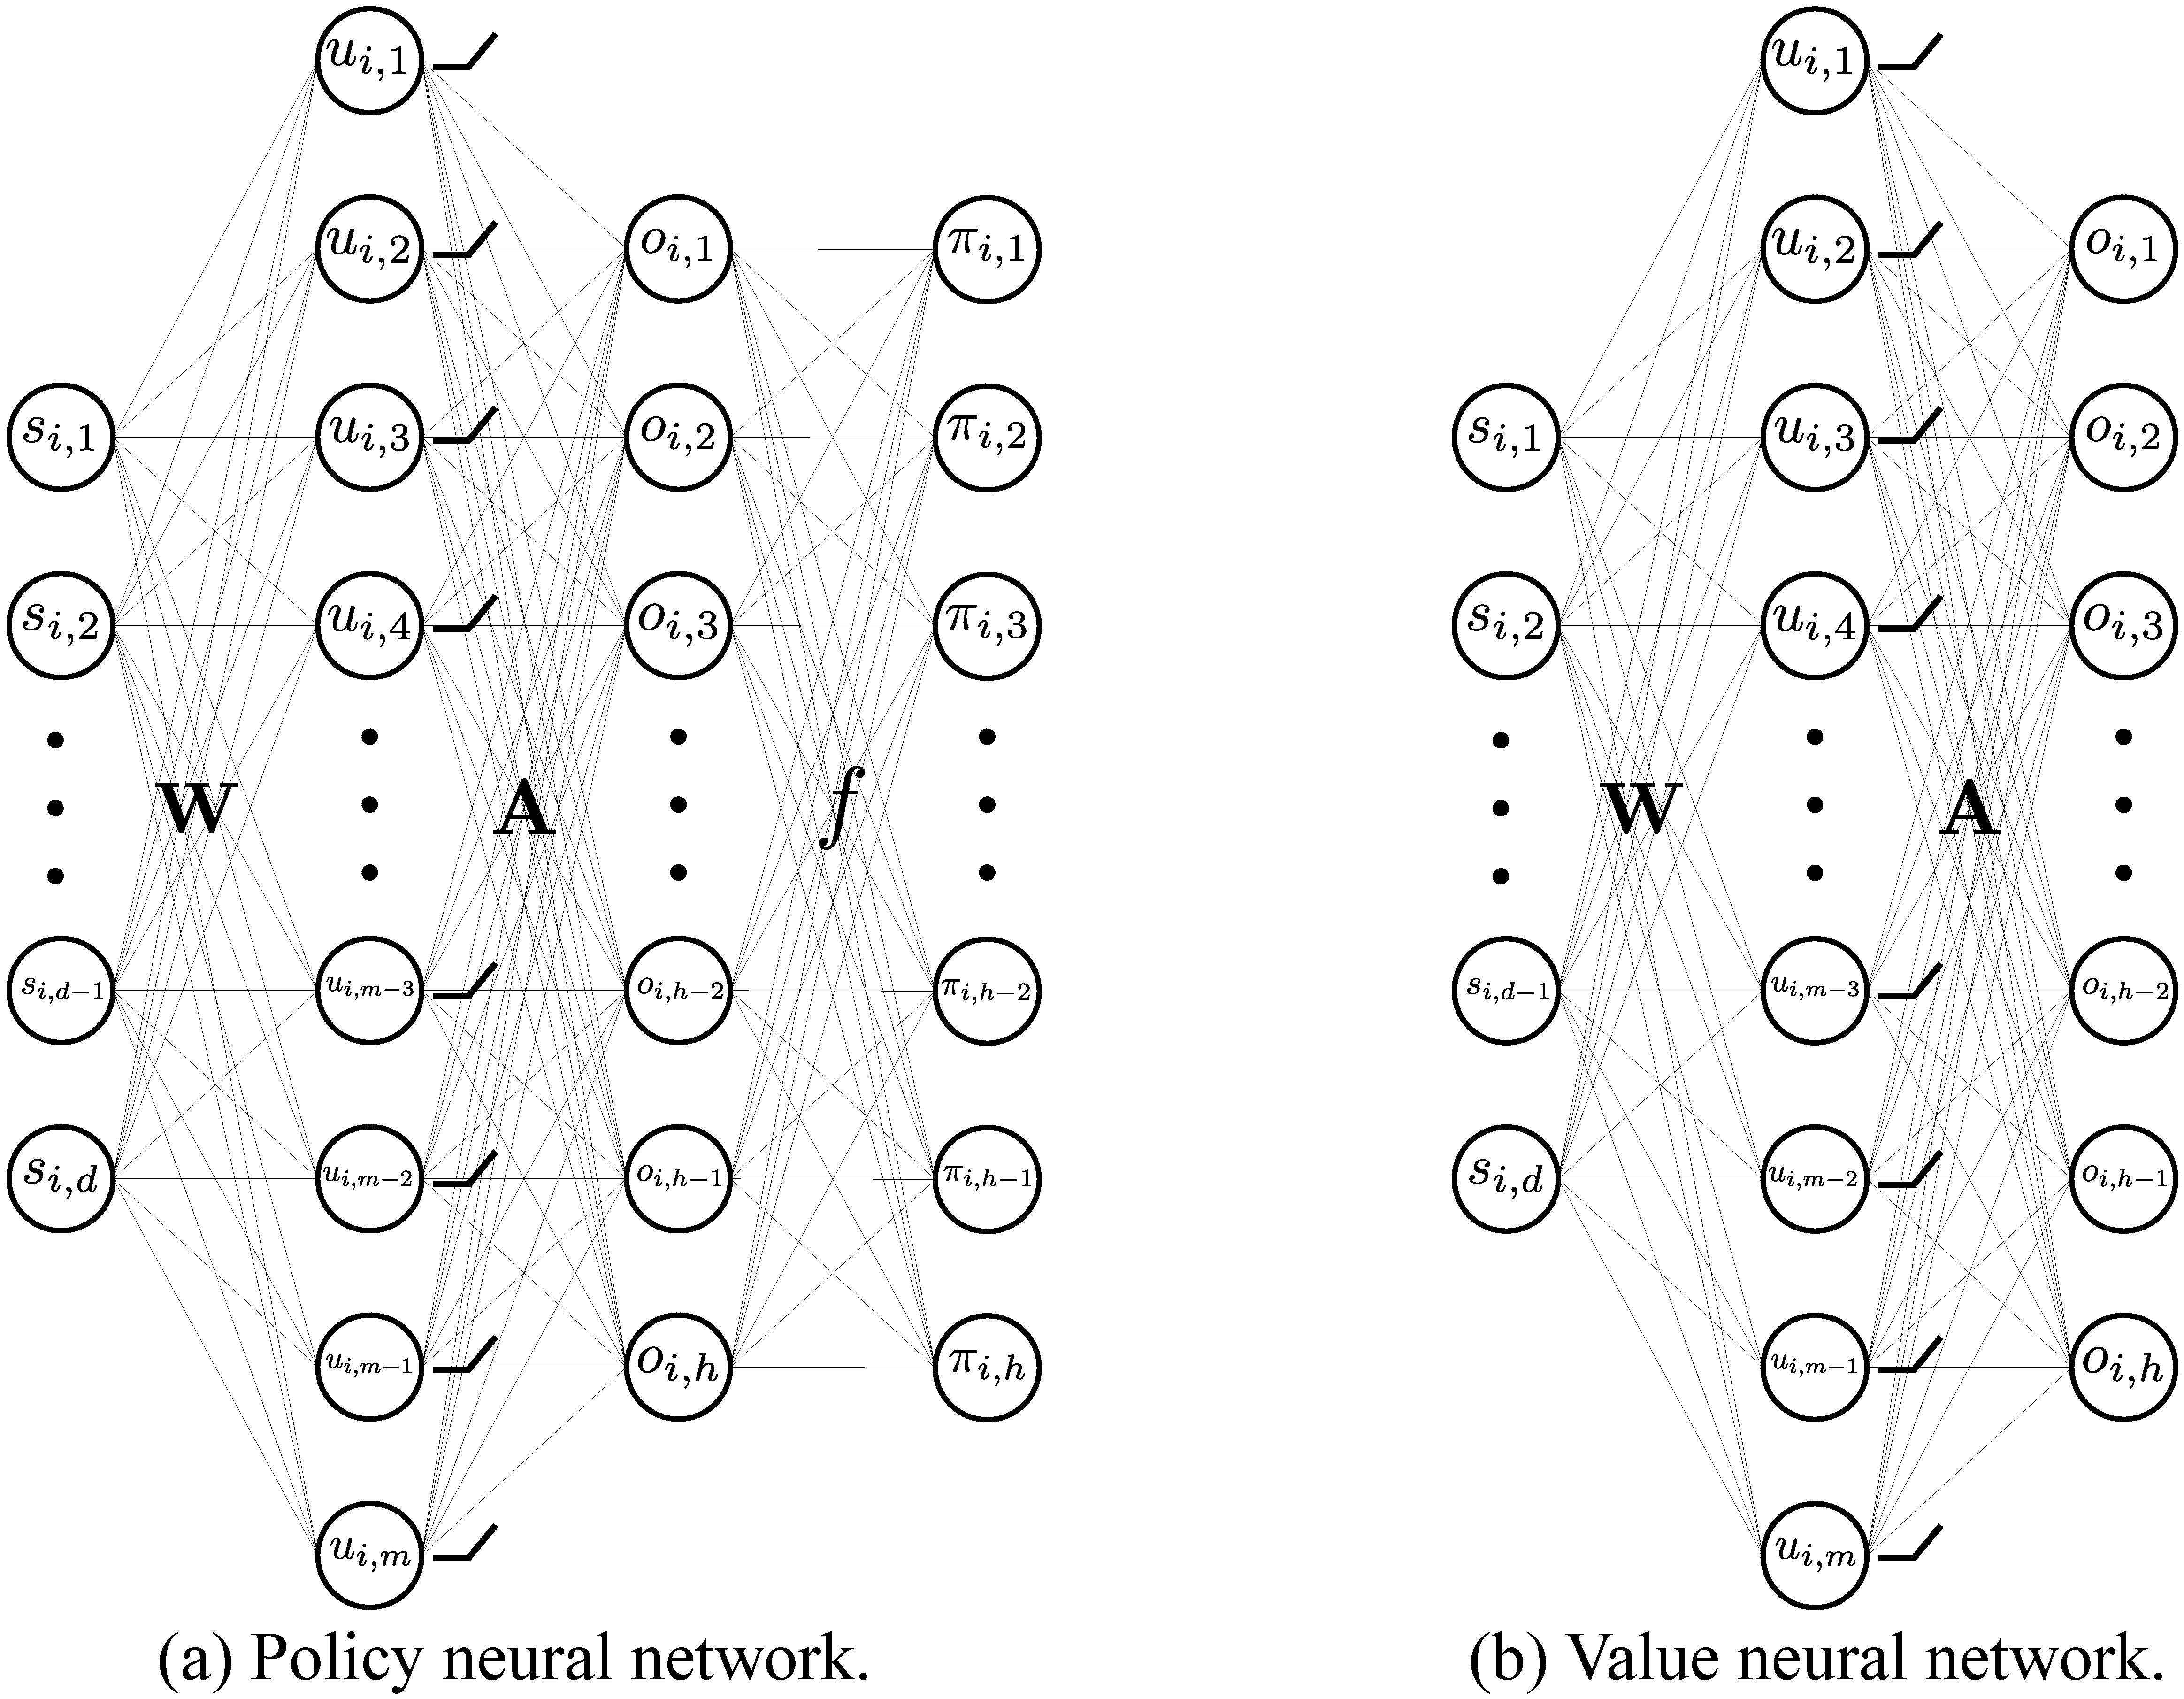
\includegraphics[width=0.8\columnwidth]{nn_policy_value_vertical.pdf}}
		\caption{The structure of the policy neural network and the value neural network.}
		\label{fig:nn_policy_value}
	\end{center}
	\vskip -0.2in
\end{figure}

We mainly focus on the stochastic bandit setting in this paper where the policy or the values of the actions are represented using a two-layer neural networks.  
However, our results can be easily generalized to many other reinforcement learning settings, e.g. state dependent stochastic bandit settings and episodic MDPs, which will be discussed in \cref{sec:general_settings}.

\subsection{Stochastic Bandit Settings}
\label{subsec:settings}

One can think of that the standard stochastic bandit setting has only one state, i.e., $n=1$.  
%At each time step $t$, the agent takes an action $A_t \in [h]$ according to its own strategies $\rvpi_t$, and then it observes a random reward $R\left(A_t\right) \in \sR$, where the mean value of $R\left(A_t\right)$ is $r\left(A_t\right)$. 
%The agent then improves its action selection strategies. 
After $T$ time steps, the performance of the agent's strategy is measured by the (expected) regret,
\begin{equation}
\label{eq:expected_regret}
R_T = \sum\limits_{t=0}^{T-1}{{\rvpi^*}^\top \rvr} - \sE \left[ \sum\limits_{t=0}^{T-1}{  r\left(A_t\right)  } \right] = \sum_{t=0}^{T-1} \sum_a \pi_t(a) \Delta(a).
%= \sum\limits_{t=0}^{T-1}{{\rvpi^*}^\top \rvr} - \sum\limits_{t=0}^{T-1}{ \sE \left[ r\left(A_t\right) \right] },
\end{equation}
where the expectation is over the randomness of action selection, if the agent is using some stochastic strategies. In the second equality, $\rvpi^*$ is a one-hot vector and $\Delta(a) = \max_b r(b)- r(a)$, and  $r(a)$ is the expected reward of the action $a$.
Without loss of generality, in this paper we assume $\rvr \in \left[ 0, 1 \right]^h$.

%\subsubsection{Episodic Markov decision process (MDP) (maybe remove this section)}
%The episodic MDP setting recovers the bandit setting as a special case. The environment randomly select a starting state $\rvs_i^0 \in \sR^d$. At each time step $t$, the agent takes one action $A_t \in [h]$ according to some strategies, and then it observes a reward $R_{i, A_t} \in \sR$ and next state $S_{t+1} \sim \sP\left( \cdot \middle| S_t, A_t \right)$, where $\sP$ is the transition probability matrix and it is unknown to the agent. After such $H$ steps, the agent observes an ending state $S_H$, and the current trajectory terminates. At the next time step, the agent will observe a new starting state $\rvs_i^0$ randomly generated by the environment. Since we use policy gradient method (no value learning), the agent updates its neural network policy weights using the cumulative reward collected after each single trajectory terminates.

%We mainly focus on the standard stochastic bandit setting with $n = 1$, i.e., there is only one state $\rvs_i$. At each time step $t$, the agent takes an action $A_t \in [h]$ according to its own strategies, and then it observes a random reward $R_{i, A_t} \in \sR$, where the mean value of $R_{i, A_t}$ is $r_{i, A_t}$. The agent then uses the reward to improve its action selection strategies. After such $T$ time steps, the performance of the agent's strategy is measured by the (expected) regret,
%\begin{equation}
%\label{eq:expected_regret}
%    \sum\limits_{t=0}^{T-1}{{\rvpi_i^*}^\top \rvr_i} - \sE \left[ \sum\limits_{t=0}^{T-1}{  r_{i, A_t}  } \right] = \sum\limits_{t=0}^{T-1}{{\rvpi_i^*}^\top \rvr_i} - \sum\limits_{t=0}^{T-1}{ \sE \left[ r_{i, A_t} \right] },
%\end{equation}
%where the expectation is over the randomness of action selection, if the agent is using some stochastic strategies.

\subsection{Policy Based and Value Based RL Methods}

Minimizing the regret \cref{eq:expected_regret} is usually formulated as the policy optimization problem, i.e., $\max\limits_{\rvpi \in \Pi}{ \expectation\limits_{ a \sim \rvpi }{ r(a)} }$, where $\Pi$ is the policy constraint. In practice, when $\Pi$ consists of all the $\rvpi\left(\rmW\right)$ represented by the parameter $\rmW$, one can use iterative gradient updates to solve the above expected reward maximization problem. This is known as the policy gradient method.

On the other hand, value based RL methods directly attempt to learn a function to approximate the value of the optimal policy, i.e., $\min\limits_{Q \in \gQ}{ \expectation\limits_{a \sim \rvb}{ \left\| Q(a) - Q^*(a) \right\|_2^2 }}$, where $\rvb$ is a behavior policy that samples actions for the learning. The learned value function induces a policy which acts greedily with respect to the value of each action.

\subsection{Neural Networks as Policy/Value Function Approximations}
\label{subsec:nn_value_policy}
 

%Both the value and the policy neural networks take the state feature  $\rvs_i \in \sR^d$ as the input. Then the networks calculate the hidden node value vector by $u_{i,r} \triangleq \rvw_r^\top \rvs_i$, $\forall r \in [m]$. The logit vector is then calculated by $o_{i,k} \triangleq \rva_k^\top \sigma\left( \rvu_i \right)$, $\forall k \in [h]$, where $\sigma$ is element-wise ReLU activation function. The value neural network outputs the logit vector $\rvo_i$. While the policy neural network output probability is the softmax transform of the logit vector, i.e., $\rvpi_i \triangleq f\left( \rvo_i \right) = f\left( \rmA \sigma\left( \rmW \rvs_i \right) \right)$. 

%The policy neural network defines a family of policies $\rvpi_i \left( \rmW \right)$ parameterized by $\rmW \in \sR^{m \times d}$ given any state $\rvs_i$. Let $\rvpi_i = \rvpi_i \left( \rmW \right)$, the expected loss of the policy neural network can be calculated according to \cref{eq:expected_loss}.

%\paragraph{Initialization of the matrix $\rmA$.} 
Without loss of generality we assume that the networks have the state $\rvs$ as their inputs satisfying $\left\| \rvs \right\|_2 = 1$.
As can be seen later, our algorithm random initializes the weight matrix $\rmA$ and fixes it during learning. 
This is a common strategy when using over-parametrized neural networks, e.g. see \citep{li2018learning,du2018gradientA,du2018gradientB,allen2018convergenceA,allen2018convergenceB}, and it has been empirically verified that there is no impact on the performance of trained neural networks \citep{hoffer2018fix}.
In this paper, each element in $\rmA$ is initialized by $a_{k,r} \sim \unif\left\{-1, +1\right\}$. Some other initializations like $\rva_k \sim \gN(0, \rmI)$ will also work. In the rest of the paper, we denote the policy $\rvpi$ by $\rvpi(\rmW_t)$ to emphasize its parametrization by $\rmW$ at time step $t$. 

%\paragraph{Multi-layered neural networks.} 
We would like to point that our algorithms and results can be extended to general value functions and policies parametrized by multi-layered neural networks resorting to related techniques \citep{allen2018convergenceA,allen2018convergenceB,du2018gradientA}. For the sake of simplicity and conciseness, we only focus on two-layers neural networks in the paper.

%Although there is only one state, i.e., $n = 1$, and $i$ can be omitted without ambiguity, we choose to keep the subscript $i$ here to make the generalization from the standard bandit setting to the many state dependent setting smoother, and our algorithms work for general $n > 1$. For simplicity, we assume $\left\| \rvs_{i} \right\|_2 = 1$, $\forall i \in [n]$.

%In the case of $n > 1$, for each state $\rvs_i$, there is a state dependent policy $\rvpi_i$. And the agent's goal is to learn totally $n$ policies using only one neural network. We assume $\left\| \rvs_{i} -  \rvs_{j} \right\|_2 \ge \delta > 0 , \ \forall i \not= j$, i.e., no duplicated data, and $\left\| \rvs_{i} \right\|_2 = 1, \ \forall i \in [n]$.


\section{Online Learning with Non-Convex Objectives and Dynamic Regret}

Online learning aims to learn changing objectives. We present general results for online learning with non-convex, smooth, gradient dominant functions.

\begin{asmp}[Bounded and smooth]
\label{asmp:boundedness_smoothness}
$\left| f_t\left(\rvx\right) \right| \le 1$, $\left\| \nabla f_t(\rvx ) - \nabla f_t(\rvy) \right\| \le L $, $\forall \rvx, \rvy$, $\forall t$.
\end{asmp}

\begin{asmp}[Gradient dominant]
\label{asmp:gradient_dominant}
$\left\| \nabla f_t\left(\rvx\right) \right\| \ge G \left[ f_t\left(\rvx\right) - \min_{\rvw}{ f_t\left(\rvw \right)} \right]$, $\forall \rvx$, $\forall t$.
\end{asmp}

\begin{defi}[Functional variation \citep{besbes2015non}]
\label{defi:function_variation}
$V_{T}^{f} \coloneqq \sum_{t=0}^{T-1}{\max\limits_{\rvw}{\left| f_{t+1}(\rvw) - f_{t}(\rvw) \right| } }.$
\end{defi}

\begin{thm}
\label{thm:online_learning_regret}
Given a sequence of functions $\left\{ f_t : t = 0, 1, 2, \dots, T-1 \right\}$ satisfying \cref{asmp:boundedness_smoothness} and \cref{asmp:gradient_dominant}. Online gradient update $\rvx_{t+1} \gets \rvx_{t} - \eta \nabla f_{t}\left(\rvx_{t}\right)$ with $\eta = 1/L$ satisfies,
\begin{equation}
\label{eq:online_learning_regret}
\begin{split}
    \sum\limits_{t=0}^{T-1}{\left[ f_t\left(\rvx_t\right) - f_t\left( \rvx_t^* \right) \right]} \le \frac{2}{G} \sqrt{L T \left( 1 + V_T^f \right)},
\end{split}
\end{equation}
where $\rvx_t^* \coloneqq \argmin_{\rvw}{f_t(\rvw)}$, $\forall t$.
\end{thm}

\cref{thm:online_learning_regret} is novel and meaningful as, (1) instead of comparing with best in hindsight $\min_{\rvw}{\sum_{t=0}^{T-1}{f_t(\rvw)} }$, we consider changing optimal decision $f_t\left( \rvx_t^* \right)$, which is more difficult to upper bound; (2) unlike most existing work, here $f_t$ is not assumed to be convex \citep{yang2016tracking} or quasi-convex \citep{gao2018online}; (3) we analyze practical gradient update; (4) our assumptions are  satisfied by randomly initialized neural networks, as justified later in next section.

To obtain sub-linear regret in \cref{eq:online_learning_regret}, it is sufficient to control the functional variation $V_T^f$ to be sub-linear $o(T)$. However, $V_T^f$ is usually linear $O(T)$ in practice. For example, in stochastic MAB, if we take sampled reward as learning signal, then at each step signal is changing in order $O(1)$ according to random sampling. As a result, $V_T^f$ will be $O(T)$. Therefore, we use empirical mean estimation and exploration to control $V_T^f$.


\section{Empirical Policy Gradient}
\label{sec:policy_gradient}

\cref{thm:online_learning_regret} shows that the variation of the learning objectives matters when gradient based methods are used in online learning. In stochastic bandit settings, to characterize the similar issue when different objectives are used for learning, we define a special functional variation, called the \textbf{reward signal variation}.

\begin{defi}[Reward signal variation]
\label{defi:reward_signal_variation}
Given a sequence of reward signals $\{ \tilde{\rvr}_t \in [0,1]^K: t = 0, 1, 2, \dots, T-1 \}$, define the reward signal variation
$V_{T}^{\tilde{\rvr}} \coloneqq \sum_{t=0}^{T-1}{\max\limits_{\rvpi \in \Delta}{\left| \rvpi^\top(\tilde{\rvr}_{t+1} - \tilde{\rvr}_{t}) \right| } } \le \sum_{t=0}^{T-1}{\left\| \tilde{\rvr}_{t+1} - \tilde{\rvr}_{t} \right\|_1  }.$
\end{defi}

Using the following example, we show that a different reward signal leads to significantly different variation.

\begin{eg}
Consider a true mean reward scalar $r \in [0, 1]$, and its two observed samples $r_t, r_{t+1} \in [0, 1]$. $\left| r_t - r_{t+1} \right| \in O(1)$ is independent with $t$, and leads to $V_T^r \in O(T)$. On the other hand, consider the empirical mean $\hat{r}_t, \hat{r}_{t+1} \in [0, 1]$, and note that
\begin{equation*}
\begin{split}
	\left| \hat{r}_{t} - \hat{r}_{t+1} \right| &\coloneqq \left| \frac{1}{t} \sum_{i=1}^{t}{ r_i } - \frac{1}{t+1} \sum_{i=1}^{t+1}{ r_i } \right| \\
	&= \frac{1}{t+1} \left| \hat{r}_t - r_{t+1} \right| \in O\left(\frac{1}{t}\right)
\end{split}
\end{equation*}
decays as $t$ increases, which leads to $V_T^{\hat{r}} \in O(\log{T})$.
\end{eg}

This simple example demonstrates that the empirical mean with sufficient exploration can obtain sub-linear reward signal variation $V_T^{\hat{r}} \in o(T)$, and is much more stable than sampled reward. Inspired by this intuition of controlling reward signal variation $V_T^{\tilde{\rvr}}$, we propose the first algorithm, Empirical Policy Gradient with Uniform Exploration (PGE), as shown in \cref{alg:policy_gradient_uniform_exploration}. Following widely used policy gradient methods, PGE updates a policy neural network by policy gradient update, but with empirical reward estimation $\hat{\rvr}_t$ as its objective. At each step $t$, PGE also has a uniform exploration $t^{ \beta - \frac{1}{3}} \cdot \frac{1}{K}$ for each action, with $\beta > 0$ to be very small. There are two main differences between PGE and standard policy gradient methods: the later uses sampled reward as the learning objective, and has no explicit exploration. In fact, the empirical mean and exploration are key components PGE uses to control $V_T^{\hat{\rvr}}$. 
 
Based on this idea, PGE achieves $\tilde{O}(T^{2/3})$ regret by balancing exploration, estimation, and online neural network learning, as shown in \cref{thm:policy_gradient_main_result}.

\begin{algorithm}[t]
\caption{Empirical Policy Gradient with Uniform Exploration (PGE)}
\label{alg:policy_gradient_uniform_exploration}
\begin{algorithmic}
   \STATE {\bfseries Input:} State feature $\rvs$, learning rate $\eta > 0$, $\beta > 0$.
   \STATE $\rvw_r(0) \sim \gN\left( 0, \sigma^2 \rmI \right)$, $\forall r \in [m]$. $a_{k, r} \sim 
   \unif\left\{-1, +1\right\}$, $\forall k \in [K]$, $\forall r \in [m]$.
   \STATE $\hat{r}_{0}(k) \gets 0$, $n_{0}(k) \gets 0$, $\tilde{\pi}_0(k) \gets \frac{1}{K}$, $\forall k \in [K]$.
   \FOR{$t=0$ {\bfseries to} $T-1$}
   \STATE Sample $A_{t} \sim \tilde{\rvpi}_{t}(\cdot | \rvs )$. Take $A_{t}$. Get reward $R_{t}$.
   \STATE $\rmW_{t+1} \leftarrow \rmW_t + \eta \cdot \frac{d \{ \rvpi_t^\top \hat{\rvr}_t \} }{d \rmW_t}$.
   \STATE $\scalemath{0.8}{ \left. 
		\begin{cases}
		n_{t+1}(k) \gets  n_{t}(k) + 1, \ \hat{r}_{t+1}(k) \gets \frac{n_{t}(k) \cdot \hat{r}_{t}(k) + R_{t} }{n_{t+1}(k)},  & \text{if } k = A_t, \\
		n_{t+1}(k) \gets n_{t}(k), \ \hat{r}_{t+1}(k) \gets \hat{r}_{t}(k),  & \text{otherwise}.
		\end{cases}
		\right.}$ 
   \STATE $\scalemath{0.75}{ \tilde{\pi}_{t+1}(k) \gets \left[ 1 - (t+1)^{ \beta - \frac{1}{3} } \right] \cdot  \pi_{t+1}(k) + (t+1)^{ \beta - \frac{1}{3} }  \cdot \frac{1}{K}, \ \forall k \in [K] }$.
   \ENDFOR
\end{algorithmic}
\end{algorithm}

\begin{thm}
	\label{thm:policy_gradient_main_result}
	Given policy neural networks as shown in \cref{fig:nn_policy_value}, with number of parameters $m \ge T^2 / K^2$, learning rate $\eta = \frac{1}{2 K m}$, $\beta = \frac{ \ln{(K/3) + \ln{\ln{t}} } }{ 3 \ln{t}}$, $\forall t \ge 2$. The expected regret of \cref{alg:policy_gradient_uniform_exploration} satisfies,
	\begin{equation*}
	\begin{split}
	\sum\limits_{t=0}^{T-1}{ ( \rvpi^* - \tilde{\rvpi}_t )^\top \rvr} \le O(T^{\frac{2}{3}}( \ln{T} )^{\frac{1}{3}}).
	\end{split}
	\end{equation*}
\end{thm}
\begin{proof}[\bf Proof sketch]
The sampling policy $\tilde{\rvpi}_t$ of PGE consists of a network policy $\rvpi_t$ and uniform exploration. Therefore, we decompose the regret into two parts,
\begin{equation}
 \label{eq:total_regret_decomposition}
 \scalemath{0.9}{
 \begin{split}
 \sum\limits_{t=0}^{T-1}{ ( \rvpi^* - \tilde{\rvpi}_t )^\top \rvr} \le \underbrace{ 2 T^{\frac{2}{3}} ( K \ln{T} )^{\frac{1}{3}} }_{\text{exploration cost}} + \underbrace{ \sum\limits_{t=1}^{T-1}{ ( {\rvpi^*} - \rvpi_t)^\top \rvr } }_{\text{NN regret}},
 \end{split}
 }
 \end{equation}
where the exploration cost is determined by summing $(t+1)^{ \beta - \frac{1}{3} }  \cdot \frac{1}{K}$. Also, because of exploration, for sufficiently large $t$, with high probability, $\hat{\rvr}_t$ will accurately estimate $\rvr$,
\begin{equation*}
    \| \hat{\rvr}_t - \rvr \|_\infty \le t^{\beta - \frac{1}{3}} \le ( K \ln{t} ) ^\frac{1}{3} t^{- \frac{1}{3}}.
\end{equation*}
The NN regret can also be decomposed as
\begin{equation}
\label{eq:playing_learning_phase_regret_decomposition}
\scalemath{0.78}{
\begin{split}
\sum\limits_{t=1}^{T-1}{ ( {\rvpi^*} - \rvpi_t )^\top \rvr}  &= \sum\limits_{t=1}^{T-1}{ ( {\rvpi^*} - \rvpi_t )^\top \hat{\rvr}_t } + \sum\limits_{t=1}^{T-1}{ ( {\rvpi^*} - \rvpi_t )^\top ( \rvr - \hat{\rvr}_t ) }\\
&\le \sum\limits_{t=1}^{T-1}{ ( {\rvpi_t^*} - \rvpi_t )^\top \hat{\rvr}_t  } + 2 \sum\limits_{t=1}^{T-1}{ \| \rvr - \hat{\rvr}_t \|_\infty } \\
&\le \underbrace{ \sum\limits_{t=1}^{T-1}{ ( {\rvpi_t^*} - \rvpi_t )^\top \hat{\rvr}_t  } }_{\text{dynamic NN regret}} + \underbrace{ O(T^{\frac{2}{3}}( \ln{T} )^{\frac{1}{3}}) }_{\text{estimation error}},
\end{split}
}
\end{equation}
where $\rvpi_t^* \coloneqq \argmax_{\rvpi }{\{ \rvpi^\top \hat{\rvr}_t\}}$. The first inequality is by $( \rvpi_t^* - \rvpi^*)^\top \hat{\rvr}_t \ge 0$ and H{\" o}lder's inequality. Next, a key step is to prove that if $m \ge T^2 /K^2$, $\eta = \frac{1}{2 K m}$, then the dynamic NN regret satisfies,
\begin{equation}
\label{step:proof1step1}
\begin{split}
\sum\limits_{t=1}^{T-1}{ (  {\rvpi_t^*} - \rvpi_t )^\top \hat{\rvr}_t } \le \frac{7 K}{c} \cdot  T^{\frac{2}{3}}
\end{split}
\end{equation}
with probability at least $1 - \frac{16 K}{T^2}$.
The regret bound follows by combining \cref{eq:total_regret_decomposition}, \cref{eq:playing_learning_phase_regret_decomposition}, and \cref{step:proof1step1}.
\end{proof}
The dynamic regret upper bound of online neural network learning \cref{step:proof1step1} is key to the proof for \cref{thm:policy_gradient_main_result}. The intuition behind \cref{step:proof1step1} is as follows. \textit{First}, we use exploration to make $\hat{\rvr}_t$ achieve sub-linear variation. In particular, with high probability, for sufficiently large $t$, every action will be visited $\Omega(t^{\frac{2}{3}})$ times, which leads to $\| \hat{\rvr}_t  - \hat{\rvr}_{t+1} \|_1 \le O(t^{-\frac{2}{3}})$. As a result, $V_T^{\hat{\rvr}} \in O(T^{\frac{1}{3}})$. \textit{Second}, we observe that expected reward satisfies \cref{asmp:boundedness_smoothness} and \cref{asmp:gradient_dominant}, which are also satisfied with high probability depending on number of neural network parameters, according to the recently developed NN optimization theory \citep{li2018learning,allen2018convergenceB}. By applying \cref{thm:online_learning_regret}, the dynamic NN regret in \cref{step:proof1step1} can be shown to be $O\left(\sqrt{T \cdot V_T^{\hat{\rvr}} }\right) \in O(T^{\frac{2}{3}})$.

\begin{remk}
The three parts for online neural network learning (exploration cost, estimation error, and dynamic regret) in the proof for \cref{thm:policy_gradient_main_result} are almost matching each other at order $\tilde{O}(T^{2/3})$, which is worse than the $\Omega(\sqrt{T})$ lower bound. However, gradient based methods with function approximation may have a lower bound that is higher than the general $\Omega(\sqrt{T})$. Whether our result is optimal remains under investigation.
\end{remk}

\iffalse
\subsection{Exploration of the Optimal Action}
\label{subsec:exploration_in_policy_learning}

Consider the logit derivative of the true mean reward,
\begin{equation}
\label{eq:logit_derivative}
\begin{split}
    \frac{d \rvpi( \rvo)^\top \rvr}{d \rvo} = \left[ \Delta(\rvpi) - \rvpi \rvpi^\top \right] \rvr,
\end{split}
\end{equation}
where $\Delta(\rvpi) \in \sR^{h \times h}$ is a diagonal matrix with $\rvpi$ as its diagonal. Suppose the $k$th action is worth learning, i.e, $r(k) - \rvpi^\top \rvr > 0$ is large, meaning this action has mean reward $r(k)$ much larger than the expected mean reward of the current policy, so the agent should increase its action logit. But if $\pi(k)$ is very close to zero, the increase of the $k$th action logit will be small. Since $\pi(k)$ is small, the $k$th action will be sampled rarely, and with other action logits increasing, $\pi(k)$ will be even smaller, which makes eventually the $k$th action cannot be sampled and learned any more.

\cref{eq:logit_derivative} indicates that to learn the $k$th action, $\pi_{t}(k) > c > 0$ should hold for some constant $c$. In particular, to learn an optimal policy, $\pi_{t}(k^*) > c > 0$ should be guaranteed, $\forall t \ge 0$, where $r(k^*) = \max\limits_{k \in \left[ h \right]}\left\{ r(k) \right\}$.

Consider policy update using \cref{eq:logit_derivative}. $\forall \eta > 0$, $\forall k \in [h]$,
\begin{equation*}
\label{eq:logit_increment_logit_space}
\begin{split}
\small
    o_{t+1}(k) - o_{t}(k) = \eta \cdot \pi_{t}(k) \cdot \left( r(k) - \rvpi(\rvo_{t})^\top \rvr \right),
\end{split}
\end{equation*}
which mean as long as $\pi_{t}(k) > 0$, for any valuable action $k$ with $r(k) -  \rvpi(\rvo_{t})^\top \rvr > 0$, the action logit will increase. While for any bad actions with $r(k) -  \rvpi(\rvo_{t})^\top \rvr < 0$, their logits will decrease.

Consider the uniform policy $\rvpi( \rvo_0)$, with $\pi_{0}(k^*) = \frac{1}{h} \in \Omega(1)$. Also note $r(k^*) - \rvpi( \rvo_0)^\top \rvr$ is larger than any other action $k$, because $k^*$ is the the optimal action. Therefore, the optimal action logit will have the largest positive increment than all the other suboptimal actions. After the softmax transform, the optimal action probability will be larger than its previous value. 
\begin{lem}
\label{lem:optimal_probability_increse_logit_space}
Policy update using \cref{eq:logit_derivative} satisfies, $\forall t \ge 0$,
\begin{equation*}
    \pi_{t+1}(k^*) \ge \pi_{t}(k^*) \in \Omega(1).
\end{equation*}
\end{lem}

\cref{alg:policy_gradient_uniform_exploration} enjoys similar results with \cref{lem:optimal_probability_increse_logit_space}. First, with enough exploration, $\hat{\rvr}_t$ is close to $\rvr$, thus $\rvpi\left(\rmW_t\right)^\top \hat{\rvr}_t$ is close to $\rvpi\left(\rmW_t\right)^\top \rvr$. Second, $\pi_{0}(\hat{k}_t^*) \approx \frac{1}{h} \in \Omega(1)$. Third, since the policy gradient update is around the initialization by \cref{lem:gradient_coupling}, the policy gradient updates behave similarly with the logit derivative updates, which makes the the optimal action logit always large comparing with the suboptimal actions.
\begin{lem}
\label{lem:optimal_probability_increse_parameter_space}
\cref{alg:policy_gradient_uniform_exploration} satisfies, $\forall t \ge 0$,
\begin{equation*}
    \pi_{t}(\hat{k}_t^*) \in \Omega(1).
\end{equation*}
\end{lem}
\cref{lem:optimal_probability_increse_parameter_space} indicates replacing $c$ in \cref{thm:policy_gradient_main_result} will not incur any additional regret dependent on $T$.
\fi


\section{Empirical Logit Learning}
\label{sec:logit_learning}

As discussed in \cref{sec:policy_gradient}, PGE achieves $\tilde{O}(T^{2/3})$ regret. One may recall that data dependent $O(\ln(T))$ regret in stochastic MAB \citep{bubeck2012regret}. A natural question is whether gradient based methods can (nearly) achieve good results.

In this section, we affirm this question by proposing an alternative algorithm, called Empirical Logit Learning with $\varepsilon$-Greedy Exploration (LLE), that is similar to value based reinforcement learning methods.

Comparing with PGE, LLE has two main differences. \textit{First}, the learning of LLE happens in the dual value/logit space, with $\ell_2$ loss $\frac{1}{2} \| \rvo_t - \hat{\rvr}_t \|^2$ as its objective. LLE takes actions based on $\rvo_t$. To get data dependent regret, $\rvo_t$ should be close to the true mean reward $\rvr$, which is not satisfied by using expected reward $\rvpi^\top \rvr$ objective. Actually, a policy $\rvpi$ with $(\rvpi^* - \rvpi)^\top \rvr = \varepsilon$ can put largest probability on the optimal arm, and there are many different ways to assign the remaining probability to sub-optimal arms. Through softmax transform, logit $\rvo$ is not guaranteed to match $\rvr$ or $\hat{\rvr}$. Therefore, we use $\ell_2$ loss as the learning objective. \textit{Second}, the reward signal in PGE satisfies $\| \hat{\rvr}_t  - \hat{\rvr}_{t+1} \|_1 \le O(t^{-\frac{2}{3}})$, and its reward signal variation is $V_T^{\hat{\rvr}} \in O(T^{\frac{1}{3}})$, which makes the learning objective stable but incurs more exploration cost. In contrast, LLE assigns much less exploration based on reward gap estimation, and its reward signal satisfies $\| \hat{\rvr}_t - \hat{\rvr}_{t+1} \|_1 \le \frac{\Delta^2}{\ln{t}}$, which means $V_T^{\hat{\rvr}} \in O(T/\ln{T})$. Directly using \cref{thm:online_learning_regret} gives undesirable regret. However, this reward signal helps $\rvo_t$ approximate $\hat{\rvr}_t$, and these two properties together suffice for convergence.

A complete algorithm is shown in \cref{alg:logit_learning_eps_greedy_exploration}. After random initialization, at each step $t$, the agent executes an $\varepsilon_t$-greedy policy, where with probability $1 - \varepsilon_t$ the agent selects action with the largest logit, or otherwise it uniformly samples an action. LLE tends to match logits with empirical mean rewards by online optimizing $\| \rvo_t - \hat{\rvr}_t\|^2$.
The exploration degree $\varepsilon_t$ is determined by estimating a lower bound, $\hat{\Delta}_t(k)$, on the reward gap between the best action and the $k$th action. This is to maintain the proper amount of exploration during learning, such that the bias $\| \hat{\rvr}_t - \rvr \|$ is small enough not to disturb the selection of the best action. Unlike in PGE, $\hat{\rvr}_t$ will not be an accurate estimation of $\rvr$. Therefore LLE cannot work in the same way of balancing exploration, estimation and learning. Finally, note that in each step, the agent only updates its value neural network using one gradient descent, therefore LLE is also in an online learning fashion.

\begin{algorithm}[t]
	\caption{Empirical Logit Learning with $\varepsilon$-Greedy Exploration (LLE)}
	\label{alg:logit_learning_eps_greedy_exploration}
	\begin{algorithmic}
		\STATE {\bfseries Input:} State feature $\rvs$, $\eta > 0$, $\alpha > 0$, $\beta > 0$.
		\STATE $\rvw_r(0) \sim \gN\left( 0, \sigma^2 \rmI \right)$, $\forall r \in [m]$. $a_{k, r} \sim \unif\left\{-1, +1\right\}$, $\forall k \in [K]$, $\forall r \in [m]$.
		\STATE $\hat{r}_{0}(k) \gets 0$, $n_{0}(k) \gets 0$, $\tilde{\pi}_t(k) \gets \frac{1}{K}$, $\ucb_{0}(k) \gets 1$, $\lcb_{0}(k) \gets 0$, $\forall k \in [K]$.
		\STATE Take every action $k$ once, update $n_{0}(k)$ and $\hat{r}_{0}(k)$.
		\FOR{$t=0$ {\bfseries to} $T-1$}
		
		\STATE Sample $A_{t} \sim \tilde{\rvpi}_t(\cdot | \rvs )$. Take $A_{t}$. Get reward $R_t$.
		\STATE $\rmW_{t+1} \leftarrow \rmW_t - \eta \cdot \frac{d \{ \frac{1}{2} \left\| \rvo_t - \hat{\rvr}_t \right\|^2 \}}{d \rmW_t}$.
		\STATE $\scalemath{0.8}{  \left. 
		    \begin{cases}
		    n_{t+1}(k) \gets n_{t}(k) + 1, \ \hat{r}_{t+1}(k) \gets \frac{n_{t}(k) \cdot \hat{r}_{t}(k) + R_t }{n_{t+1}(k)}, & \text{if } k = A_t, \\
		    n_{t+1}(k) \gets n_{t}(k), \ \hat{r}_{t+1}(k) \gets \hat{r}_{t}(k), & \text{otherwise}.
		    \end{cases}
		    \right. }$
		%\STATE $n_{t+1}\left(A_t\right) \gets n_{t}\left(A_t\right) + 1$.
		%\STATE $n_{t+1}(k) \gets n_{t}(k)$, $\forall k \not= A_t$.
		%\STATE $\hat{r}_{t+1}\left(A_t\right) \gets \frac{n_{t}\left(A_t\right) \cdot \hat{r}_{t}\left(A_t\right) + R_{A_{t}}\left(n_{t}\left(A_t\right)\right) }{n_{t+1}\left(A_t\right)}$.
		%\STATE $\hat{r}_{t+1}(k) \gets \hat{r}_{t}(k)$, $\forall k \not= A_t$.
		\STATE $\scalemath{0.75}{ \ucb_{t+1}(k) \gets
		    \min{\left\{ 1, \hat{r}_{t+1}(k) + \sqrt{\frac{\alpha \ln{( (t+1) K^{\frac{1}{\alpha}})}}{2 n_{t+1}(k)}}\right\}}, \ \forall k \in [K] }$.
		%\STATE $\ucb_{t+1}\left(A_t\right) \gets \min{\left\{ 1, \hat{r}_{t+1}\left(A_t\right) + \sqrt{\frac{\alpha \ln{\left( t h^{\frac{1}{\alpha}}\right)}}{2 n_{t+1}\left(A_t\right)}}\right\}}$.
		%\STATE $\ucb_{t+1}(k) \gets \ucb_{t}(k)$, $\forall k \not= A_t$.
		\STATE $\scalemath{0.75}{ \lcb_{t+1}(k) \gets 
		    \max{\left\{ 0, \hat{r}_{t+1}(k) - \sqrt{\frac{\alpha \ln{( (t+1) K^{\frac{1}{\alpha}})}}{2 n_{t+1}(k)}}\right\}}, \ \forall k \in [K] } $.
		%\STATE $\lcb_{t+1}\left(A_t\right) \gets \max{\left\{ 0, \hat{r}_{t+1}\left(A_t\right) - \sqrt{\frac{\alpha \ln{\left( t h^{\frac{1}{\alpha}}\right)}}{2 n_{t+1}\left(A_t\right)}}\right\}}$.
		%\STATE $\lcb_{t+1}(k) \gets \lcb_{t}(k)$, $\forall k \not= A_t$.
		
		\STATE $\scalemath{0.8}{ \hat{\Delta}_{t+1}(k) \gets \min\left\{ 1,  \min\limits_{k^\prime \in \left[K\right]}\left\{ \lcb_{t+1}(k^\prime) \right\}  - \ucb_{t+1}(k)\right\}, \ \forall k \in [K] }  $.
		\STATE $\scalemath{0.65}{ \xi_{t+1}(k) \gets \frac{\beta \ln{(t+1)}}{(t+1) \hat{\Delta}_{t+1}^2(k)}, \ \varepsilon_{t+1}(k) \gets \min\left\{ \frac{1}{2 K}, \frac{1}{2} \sqrt{\frac{\ln{K}}{(t+1) K}},  \xi_{t+1}(k) \right\} }$.
		\STATE $\scalemath{0.9}{ \pi_{t+1}(k) \gets \left. 
		    \begin{cases}
		    1, & \text{if } k = \argmax\limits_{k^\prime \in \left[K\right]}\left\{ o_{t+1}(k^\prime)\right\}, \\
		    0, & \text{otherwise}.
		    \end{cases}
		    \right. }$
		%\STATE $\pi_{t}(k) \gets 1$, for $k = \argmax\limits_{k^\prime \in \left[h\right]}\left\{ o_{t}(k^\prime)\right\}$.
		%\STATE $\pi_{t}(k) \gets 0$, $\forall k \not= \argmax\limits_{k^\prime \in \left[h\right]}\left\{ o_{t}(k^\prime)\right\}$.
		\STATE $\scalemath{0.8}{ \tilde{\pi}_{t+1}(k) \gets \left[ 1 - \sum\limits_{k^\prime \in [h]}{\varepsilon_{t+1}(k)} \right] \cdot  \pi_{t+1}(k) + \varepsilon_{t+1}(k)$, $\forall k \in [K] }$.
		
		\ENDFOR
	\end{algorithmic}
\end{algorithm}

%\subsection{Theoretical analysis}
%\label{subsec:theoretical_analyses_logit_learning}

%It seems difficult to improve \cref{thm:policy_gradient_main_result}, as all the three parts of the regret are almost balanced, i.e., uniform exploration ($ T^{\frac{2}{3} + \beta}$, \cref{eq:total_regret_decomposition}), estimation error ($ T^{\frac{2}{3} + \beta} $, \cref{thm:reward_estimation_hoeffding}), and the cumulative expected loss of neural network policies ($ T^{\frac{2}{3} - \frac{\beta}{2}} $, \cref{thm:dynamic_regret_sublinear}). \cref{alg:policy_gradient_uniform_exploration} learns policies in the primal policy space by maximizing $\rvpi\left( \rmW_t \right)^\top \hat{\rvr}_t$. And it is not necessary that $\rvo\left( \rmW_t\right)$ is close to $\hat{\rvr}_t$, due to the homogeneity invariant property of the softmax, i.e, $\rvpi\left(\rvo + a \cdot \rvone \right) = \rvpi(\rvo)$, $\forall a \in \sR$. To show the convergence of $\rvpi\left( \rmW_t \right)^\top \hat{\rvr}_t$, every action needs to be pulled many times, which leads to the undesirable regret results.


The next theorem shows that LLE has a nearly optimal regret rate in the stochastic MAB setting.
\begin{thm}
\label{thm:logit_learning_main_result}
    Given value neural networks as shown in \cref{fig:nn_policy_value}, with number of hidden nodes $m \ge T^2 / K^2$, learning rate $\eta = \frac{1}{K m}$,  $\alpha > 3$, and $\beta > 256$, the expected regret of \cref{alg:logit_learning_eps_greedy_exploration} satisfies,
\begin{equation*}
\begin{split}
    \sum\limits_{t=0}^{T-1}{ ( {\rvpi^*} - \tilde{\rvpi}_t)^\top \rvr } \le \sum\limits_{\Delta(k) > 0}{ \left[ \frac{ 3 \beta ( \ln{T} )^2}{\Delta^2(k)} \right] }  + 3 \ln{T} + C,
\end{split}
\end{equation*}
%where $C \triangleq 2 \max\limits_{k \in [h]}\left\{ \bar{t}(k) \right\} + \pi^2$ is independent with $T$.
where $C$ is a constant independent with $T$.
\end{thm}
\begin{proof} [\bf Proof sketch]
		By Proposition 2 of \citet{seldin2017improved}, $\hat{\Delta}_t(k)$ is a valid estimate of reward gap $\Delta(k)$, in the sense that for large enough $t$ with high probability, 
		\begin{equation*}
		    \Delta(k)/2 \le \hat{\Delta}_t(k) \le 	\Delta(k).
		\end{equation*}
		Now given a proper estimate of $\Delta(k)$, note the exploration portion is set to be $\frac{\beta\ln t}{t \hat{\Delta}^2(k)}$.
		We can further show that with high probability each action is sampled at least $\frac{25 \ln t}{\Delta^2(k)}$ times with a large enough $\beta$, and therefore with high probability, $\forall k \in [K]$, 
		\begin{equation*}
		    | \hat{r}_t(k) - r(k) | \le \Delta(k)/5.
		\end{equation*}
		The key of our proof is to show that the learning loss 
		\begin{equation*}
		    \| \rvo_t - \hat{\rvr}_{t}\| \le \Delta(k)/5, \quad \forall k \in [K].
		\end{equation*}
		for large enough $t$. Therefore $\forall k \in [K]$,
		\begin{equation*}
		    | o_t(k) - r(k) | \le \| \rvo_t - \hat{\rvr}_t\| + | \hat{r}_t(k) - r(k) | \le 2\Delta(k)/5,
		\end{equation*}
		i.e., the agent will select the optimal action by greedily acting on value network output $\rvo_t$. To show that, note 
		\begin{equation*}
		\scalemath{0.7}{
		\begin{split}
		\frac{1}{2} \| \rvo_{t+1} - \hat{\rvr}_{t+1}\|^2 &= \frac{1}{2} \| \rvo_{t+1} - \hat{\rvr}_t\|^2 + ( \rvo_{t+1} - \hat{\rvr}_t )^\top ( \hat{\rvr}_t - \hat{\rvr}_{t+1} ) + \frac{1}{2} \| \hat{\rvr}_t - \hat{\rvr}_{t+1} \|^2 \\
		&\le \frac{1}{2} \| \rvo_{t+1} - \hat{\rvr}_t\|^2 + \| \rvo_{t+1} - \hat{\rvr}_t\| \cdot \frac{\Delta^2(k)}{\ln{t}} + \frac{\Delta^4(k)}{2 ( \ln{t} )^2 },
		\end{split}
		}
		\end{equation*}
		where the last inequality is by $\| \hat{\rvr}_t - \hat{\rvr}_{t+1} \|_2 \le \frac{\Delta^2(k)}{\ln{t}}$ because $\hat{\rvr}_t$  and $\hat{\rvr}_{t+1}$ are two consecutive empirical means and each action has been selected at least $\frac{\ln t}{\Delta^2(k)}$ times. Denote $\delta_t = \| \rvo_t - \hat{\rvr}_{t}\|$. Combining with \cref{lem:logit_l2_loss_parameter_smoothness},
		\begin{equation*}
		    \delta_{t+1} \le \sqrt{1 - \frac{1}{2 K} } \cdot \delta_{t} + \frac{\Delta^2(k)}{\ln{t}},
		\end{equation*}
		based on which one can further show that $\delta_t \le \Delta(k) / 5$ for large enough $t$. Finally, the probability of selecting a sub-optimal action can be bounded by the sum of the exploration probability and the probability of the rare event when not all the above claims hold, which leads to an upper bound on the expected regret.
		\end{proof}
	\begin{lem}
		\label{lem:logit_l2_loss_parameter_smoothness}
		$\rmW_{t+1} \gets \rmW_t - \eta \cdot \frac{d \{ \frac{1}{2} \| \rvo_t - \hat{\rvr}_t \|^2 \}}{d \rmW_t}$, with $\eta = \frac{1}{K m}$. With high probability, $\forall t \le \frac{\tau}{2 \eta} \coloneqq \frac{1}{2 \eta \sqrt{m}}$, 
		\begin{equation*}
		\begin{split}
		\frac{1}{2} \| \rvo_{t+1} - \hat{\rvr}_t \|^2 \le \left( 1 - \frac{1}{2 K} \right) \cdot \frac{1}{2} \| \rvo_t - \hat{\rvr}_t \|^2.
		\end{split}
		\end{equation*}
	\end{lem}
	
\begin{remk}
	The $O((\ln T)^2)$ regret of LLE is worse than the optimal rate $O(\ln T)$. 
	This is due to low efficiency of $\varepsilon$-greedy exploration.
	In particular, to have a proper $\varepsilon$, one needs to estimate the reward gaps $\Delta(k)$, which causes the extra $\ln T$ factor.
	A UCB style of exploration that requires no knowledge about the reward gaps may be able to reduce this extra $\ln T$ factor.
\end{remk}



\section{General Settings}
\label{sec:general_settings}

===============updated:jincheng
Although the stochastic bandit setting is an oversimplified RL environment, it captures the trade off between exploration and exploitation, which is the intrinsic nature of many more complicated RL tasks. Beyond the stochastic bandit setting, our results can be easily generalized to the following more general settings with minimal efforts.

\subsection{Episodic Markov Decision Processes (MDPs)}

Each action in the standard bandit setting can be viewed as a special trajectory with length $H = 1$ in the episodic MDPs. In general with $H > 1$, \cref{alg:logit_learning_eps_greedy_exploration} can achieve similar result, with the total trajectory number changing from $h$ to $h^H$.
\begin{thm}
\label{thm:episodic_mdp_setting}
     Suppose $m \in \Theta\left( \frac{T^2}{c^4 h^{2H}} \right)$, $\eta = \frac{ 1 }{16 h m}$, the expected regret of \cref{alg:logit_learning_eps_greedy_exploration} satisfies $\sum\limits_{t=0}^{T-1}{ \left( {\rvpi^*}^\top \rvr - \sE \left[ r\left(A_t\right) \right] \right) } \le \sum\limits_{k \in [h^H] : \Delta(k) > 0}{ \left[ \frac{ 3 \beta \left( \ln{T} \right)^2}{\Delta^2(k)} \right] } + 3 \ln{T} + C$, where $C$ is constant of $T$.
\end{thm}

The number of terms in the summation has an undesirable exponential dependence of trajectory length $H$. This seems cannot be eliminated by policy based RL methods, without taking advantage of the intermediate rewards in value based RL methods, such as Q-Learning \citep{jin2018q}. It is open whether value based RL methods enjoy nice theoretical guarantees with neural network function approximations.

\subsection{State Dependent Bandit Setting}

The standard stochastic bandit setting is a special case of the many state dependent bandit setting, with $n = 1$. Firstly, all the intermediate results work for general $n > 0$, including the $n > 1$ case.
For $n > 1$ and $\delta \triangleq \min{\left\| \rvs_i - \rvs_j \right\|} > 0$, we slightly modify \cref{alg:logit_learning_eps_greedy_exploration}, by setting the objective as the sum of all the $n$ terms. Consider the average expected loss over all the states, the regret results are similar with \cref{thm:logit_learning_main_result}, up to an additional factor $n$, can be easily reproduced.
\begin{thm}
\label{thm:many_state_dependent_bandit_setting}
     Suppose $m \in \Theta\left( \frac{n^{10} T^2}{c^4 \delta^4 h^2} \right)$, $\eta = \frac{c^2 \delta^2}{16 n^4 h m}$, the expected regret of \cref{alg:logit_learning_eps_greedy_exploration} satisfies $\frac{1}{n } \sum\limits_{i=1}^{n}{ \sum\limits_{t=0}^{T-1}{ \left( {\rvpi_i^*}^\top \rvr_i - \sE \left[ r_i\left(A_{i,t}\right) \right] \right) } \le \sum\limits_{k \in [h] : \Delta_i(k) > 0}{ \left[ \frac{ 3 \beta n^8 \left( \ln{T} \right)^2}{c^4 \delta^4 \Delta_i^2(k)} \right] } + 3 n \ln{T} + C }$.
\end{thm}




\section{Future Work}
\label{sec:future_work}

Our results are just at the beginning of theoretically understanding DRL. There are many problems remain open along this line.
\begin{itemize}
    \item The first open problem would be a policy based algorithm that can achieve $O(\ln T)$ regret. \cref{alg:policy_gradient_uniform_exploration} only achieves a $\tilde{O}(T^{2/3})$ regret. We hypothesize that a better rate should be achievable with a better analysis and less exploration in \cref{alg:policy_gradient_uniform_exploration}. 
    Especially such better analysis should be able to leverage the property that the algorithm needs not to have an small estimation error $\|\hat{\rvr} - \rvr\|_\infty$ to pick the optimal action.
    \item In this paper we only consider the $\varepsilon$-greedy for exploration, which may not be optimal. Other exploration strategies, like count based exploration \cite{auer2002finite}, EXP3 \citep{seldin2014one}, posterior sampling \citep{agrawal2012analysis} 
    may be able to improve the current regret rates. Especially, with other type of explorations, can \cref{alg:logit_learning_eps_greedy_exploration} be improved to achieve an $O(\ln T)$ regret.
    \item Our algorithms memorize the empirical mean reward for each pair of state and action, which is not viable for large scale problems in practice. Instead, most of the practical RL algorithms use the sampled reward at the current step, instead of the empirical mean, as an approximation of the true reward. Can we still prove similar regrets for the current reward.
    \item In practice, gradient updates always travel a long distance rather than around initialization \citep{liu2018deeptracker}. And usually, practical NNs do not have that much overparametrized scales. Further progresses in the DL theory would be helpful for improving our current analyses of DRL.
    \item One interpretation of the last softmax layer could be from the maximum entropy policy optimization, where the softmax is the solution of the entropy regularized reward maximization \cite{nachum2017bridging}. In this perspective, mirror descent seems to be a more natural optimizer compared to gradient descent. Could a mirror descent optimizer lead to a better regret rate in our setting?
    \item We have just investigated the vanilla policy based and value based algorithms. Can our results be extended to other successful RL algorithms including value based and actor critic methods, e.g., DQN \citep{mnih2015human}, A3C \citep{mnih2016asynchronous}, and PCL \citep{nachum2017bridging}, etc.
    %\item For policy leaning with NN function approximations, there is no known lower bound, although at least the general $\Omega\left(\sqrt{T}\right)$ lower bound holds. We can get some sense from the two parts of the regret in \cref{thm:policy_gradient_main_result}. The NN learning part seems cannot be improved, since this is the best one can obtain under smoothness like properties and gradient upper $\&$ lower bounds. While the other exploration and estimation error part seems still have space to be improved. But whether $\Omega\left(\sqrt{T}\right)$ is achievable is still unknown.
\end{itemize}

\if0
% In the unusual situation where you want a paper to appear in the
% references without citing it in the main text, use \nocite
\nocite{langley00}
\fi

\section{Conclusions}
\label{sec:conclusions}
We proved a $\tilde{O}(T^{2/3})$ regret for a vanilla policy based reinforcement learning algorithm under the stochastic multi-armed bandit setting. 
Noticing the main hurdle in our proof as the estimation error $\|\hat{\rvr} - \rvr\|$, we further proposed a value based RL algorithm, Logit Learning with $\varepsilon$-Greedy Exploration (LLE). 
We proved that LLE achieve a nearly optimal regret $O((\ln T)^2)$.
Our results can be generalized to many state dependent bandit settings, episodic MDPs, and can be combined with multi-layered neural network function approximations. Our findings are at the starting point of understanding more perspectives and providing theoretical supports for deep reinforcement learning. We also discussed several open problems for future research.

\bibliography{aistats2020}
\bibliographystyle{iclr2020_conference}

\onecolumn
\section{Proofs}

{\bf \cref{lem:equivalence_ment_reinforce}.} Using importance sampling in \cref{alg:erpg_ment_reinforce},
\begin{equation*}
    \nabla{(\rvtheta_t)} = \expectation\limits_{\rho \sim \rvpi_t}{ \left( \rvr_t(\rho) - \log{\rvpi_t(\rho)} \right) \cdot \nabla{ \log{\rvpi_t(\rho)} } }, \quad \forall t \ge 1.
\end{equation*}
\begin{proof}
According to the gradient definition in \cref{alg:erpg_ment_reinforce}, $\forall t \ge 1$,
\begin{equation*}
\begin{split}
    \nabla{(\rvtheta_t)} &= \frac{d \left\{ \rvpi(\rvo_t)^\top \rvr_t - \rvpi(\rvo_t)^\top \log{\rvpi(\rvo_t)} \right\} }{d \rvtheta_t} \\
    &= \left( \frac{d \rvpi_t}{d \rvo_t} \right)^\top \left( \rvr_t - \rvone - \log{\rvpi_t} \right) \\
    &= \left( \frac{d \rvpi_t}{d \rvtheta_t} \right)^\top \left( \rvr_t - \log{\rvpi_t} \right) \\
    &= \left( \frac{d \rvpi_t}{d \rvtheta_t} \right)^\top \left[ \sum\limits_{i \in [K]}{ \rvpi_t(i) \cdot \rvone_{ \left\{ \frac{\rvr_t(i) - \log{\rvpi_t(i)} }{\rvpi_t(i)} \right\} } } \right]  \\
    &= \sum\limits_{i \in [K]}{ \rvpi_t(i) \cdot \left[ \left( \frac{d \rvpi_t}{d \rvtheta_t} \right)^\top \rvone_{ \left\{ \frac{\rvr_t(i) - \log{\rvpi_t(i)} }{\rvpi_t(i)} \right\} } \right] } \\
    &= \sum\limits_{i \in [K]}{ \rvpi_t(i) \cdot \left[ \frac{\rvr_t(i) - \log{\rvpi_t(i)} }{\rvpi_t(i)} \cdot \frac{d \rvpi_t(i)}{d \rvtheta_t}  \right] } \\
    &= \expectation\limits_{\rho \sim \rvpi_t}{ \left( \rvr_t(\rho) - \log{\rvpi_t(\rho)} \right) \cdot \nabla{ \log{\rvpi_t(\rho)} } }. \qedhere
\end{split}
\end{equation*}
\end{proof}

\begin{lem}
Let $\rvr_1, \rvr_2, \dots, \rvr_t \in \left[ 0, 1  \right]^K$. Denote $\rvr_{1:t} \triangleq \sum\limits_{i=1}^{t}{\rvr_i}$, and $\hat{\rvr}_t \triangleq \frac{\rvr_{1:t}}{t}$. Let $\rvo \in \sR^K$ be any logit vector, and $\rvpi(\rvo) \triangleq \softmax(\rvo)$ be the softmax policy of $\rvo$. For any policy $\rvpi$, define $\rmH\left( \rvpi \right) \triangleq \Delta \left( \rvpi \right) - \rvpi \rvpi^\top$, where $\Delta \left( \rvpi \right) \in \sR^{K \times K}$ is a diagonal matrix, with $\rvpi$ as its diagonal. Define the entropy regularized policy gradient with respect to logit at step $t$,
\begin{equation*}
\begin{split}
    \nabla(\rvo_t) &\triangleq \frac{d \left\{ \rvpi(\rvo_t)^\top \rvr_t - \rvpi(\rvo_t)^\top \log{\rvpi(\rvo_t)} \right\} }{d \rvo_t} \\
    &= \left[ \Delta \left( \rvpi(\rvo_t) \right) - \rvpi(\rvo_t) \rvpi(\rvo_t)^\top \right] \left( \rvr_t - \rvo_t \right).
\end{split}
\end{equation*}
Denote $\rmH_t \triangleq \rmH(\rvpi(\rvo_t))$.
Consider the entropy regularized policy gradient update,
\begin{equation*}
\begin{split}
    \rvo_{t+1} &= \rvo_t + \eta \cdot \nabla(\rvo_t) \\
    &= \rvo_t + \eta \cdot \rmH_t \left( \rvr_t - \rvo_t \right).
\end{split}
\end{equation*}
If the learning rate $\eta$ at iteration $t$ satisfies
\begin{equation*}
\begin{split}
    \eta \ge \frac{ \frac{1}{t+1} + \frac{1}{(t+1)(t+C)} }{ \frac{1}{e K} \cdot \left( 1 - \frac{2 C \sqrt{K}}{t+1} \right)  } = e K \cdot \left( 1 + \frac{1}{t+C} \right) \cdot \frac{1}{t+1-2C\sqrt{K}} = O\left( \frac{1}{t} \right),
\end{split}
\end{equation*}
then there exists a scalar $c_t \in \sR$, such that
\begin{equation*}
    \left\| \rvo_{t+1} - \hat{\rvr}_{t} + c_t \rvone \right\| \le \frac{C \sqrt{K}}{t+1}, \quad \forall t \ge 0.
\end{equation*}
\end{lem}
\begin{proof}
We use induction on $t$. For $t=0$, and $c_0 = 0$,
\begin{equation*}
\begin{split}
    \left\| \rvo_{1} - \hat{\rvr}_0 + c_0 \rvone \right\| = \left\| \rvzero \right\| = 0 \le C \sqrt{K}.
\end{split}
\end{equation*}
Assume $\left\| \rvo_{t} - \hat{\rvr}_{t-1} + c_{t-1} \rvone \right\| \le \frac{C \sqrt{K}}{t}$ for some $t \ge 1$. There  are two different cases of the update.

\textbf{First case:} $\rvr_t - \rvo_t = a_t \rvone$, where $a_t \in \sR$. This means $\rvo_{t+1} = \rvo_{t}$. Let $c_t \triangleq \frac{(t-1)c_{t-1}}{t} +  \frac{a_t}{t}$, we have
\begin{equation*}
\begin{split}
    \left\| \rvo_{t+1} - \hat{\rvr}_t + c_t \rvone \right\| &= \left\| \rvo_{t} - \hat{\rvr}_t + \frac{(t-1)c_{t-1}}{t} \rvone + \frac{a_t}{t} \rvone \right\| \\
    &= \left\| \rvo_{t} - \frac{\rvr_{1:t-1} + \rvr_t}{t-1} \cdot \frac{t-1}{t} + \frac{(t-1)c_{t-1}}{t} \rvone + \frac{a_t}{t} \rvone \right\| \\
    &= \left\| \rvo_{t} - \hat{\rvr}_{t-1} + \frac{\hat{\rvr}_{t-1}}{t} - \frac{\rvo_t + a_t \rvone}{t} + \frac{(t-1)c_{t-1}}{t} \rvone + \frac{a_t}{t} \rvone \right\| \\
    &= \left\| \frac{t-1}{t} \cdot \left( \rvo_{t} - \hat{\rvr}_{t-1} + c_{t-1} \rvone \right) \right\| \\
    &\le \frac{t-1}{t} \cdot \frac{C \sqrt{K}}{t} \\
    &\le \frac{C \sqrt{K}}{t+1}.
\end{split}
\end{equation*}

\textbf{Second case:} $\rvr_t - \rvo_t \not= a_t \rvone$, for any $a_t \in \sR$. Then $\rvo_{t+1} \not= \rvo_t$. By the inductive hypothesis,
\begin{equation*}
\begin{split}
    \left| \rvo_{t}(i) - \hat{\rvr}_{t-1}(i) + c_{t-1} \right| \le \left\| \rvo_{t} - \hat{\rvr}_{t-1} + c_{t-1} \rvone \right\| \le \frac{C \sqrt{K}}{t}, \quad \forall i \in [K].
\end{split}
\end{equation*}
Denote $i_{\min} \triangleq \argmin\limits_{i \in [K]}{\rvo_t(i)} $, $i_{\max} \triangleq \argmax\limits_{i \in [K]}{\rvo_t(i)} $, and $\gF(\rvo_t) \triangleq \log{\sum\limits_{i = 1}^K{\exp\left\{ \rvo_t(i) \right\}} } \le \rvo_t(i_{\max}) + \log{K}$. The smallest probability of $\rvpi_t$ can be lower bounded as
\begin{equation*}
\begin{split}
    \min\limits_{i \in [K]}{\rvpi_t(i)} &= \min\limits_{i \in [K]}{ \exp\left\{ \rvo_t(i) - \gF(\rvo_t) \right\} } \\
    &= \exp\left\{ \min\limits_{i \in [K]}{\rvo_t(i)} - \gF(\rvo_t) \right\} \\
    &\ge \exp\left\{ \rvo_t(i_{\min}) - \rvo_t(i_{\max}) - \log{K} \right\} \\
    &\ge \exp\left\{ \hat{\rvr}_{t-1}(i_{\min}) - \frac{C \sqrt{K}}{t} - \hat{\rvr}_{t-1}(i_{\max}) - \frac{C \sqrt{K}}{t} - \log{K} \right\} \\
    &\ge \exp\left\{ -1 - \log{K} - \frac{2 C \sqrt{K}}{t} \right\} \\
    &= \frac{1}{e K} \cdot \exp\left\{ - \frac{2 C \sqrt{K}}{t} \right\} \\
    &\ge \frac{1}{e K} \cdot \left( 1 - \frac{2 C \sqrt{K}}{t} \right).
\end{split}
\end{equation*}
Using the choice of learning rate $\eta$ at step $t$,
\begin{equation*}
\begin{split}
    \eta \cdot \lambda_{\min}^{+}\left\{ \rmH_t \right\} &\ge \eta \cdot \min\limits_{i \in [K]}{\rvpi_t(i)} \\
    &\ge \eta \cdot \frac{1}{e K} \cdot \left( 1 - \frac{2 C \sqrt{K}}{t} \right) \\
    &\ge \frac{1}{t+1} + \frac{1}{(t+1)(t+C)}.
\end{split}
\end{equation*}
Let $c_{t} = c_{t-1}$. According to the update,
\begin{equation*}
\begin{split}
    \rvo_{t+1} - \hat{\rvr}_t + c_{t} \rvone &= \rvo_{t} - \hat{\rvr}_{t-1} + c_{t-1} \rvone + \hat{\rvr}_{t-1} - \hat{\rvr}_t - \eta \cdot \rmH_t \left( \rvo_{t} - \hat{\rvr}_{t-1} + c_{t-1} \rvone \right) - \eta \cdot \rmH_t \left( \hat{\rvr}_{t-1} - \rvr_t \right).
\end{split}
\end{equation*}
Denote $\rvdelta_{t} \triangleq \rvo_{t} - \hat{\rvr}_{t-1} + c_{t-1} \rvone$. Note that
\begin{equation*}
\begin{split}
    \hat{\rvr}_{t-1} - \hat{\rvr}_t &= \frac{\rvr_{1:t-1}}{t-1} - \frac{\rvr_{1:t-1} + \rvr_t}{t} = \frac{\rvr_{1:t-1} - (t-1) \cdot \rvr_t }{t(t-1)} = \frac{1}{t} \cdot \left( \hat{\rvr}_{t-1} - \rvr_t \right).
\end{split}
\end{equation*}
We have the following iterative relation,
\begin{equation*}
\begin{split}
    \rvdelta_{t+1} = \left[ \rmI - \eta \cdot \rmH_t \right] \rvdelta_t + \left[ \frac{1}{t} \cdot \rmI - \eta \cdot \rmH_t \right] \left( \hat{\rvr}_{t-1} - \rvr_t \right).
\end{split}
\end{equation*}
By the triangle and H{\" o}lder's inequality, assuming $\rvdelta_t \not= b_t \rvone$ and $\hat{\rvr}_{t-1} - \rvr_t \not= d_t \rvone$ for any $b_t, d_t \in \sR$,
\begin{equation*}
\begin{split}
    \left\| \rvdelta_{t+1} \right\| &\le \lambda_{\max}\left\{ \rmI - \eta \cdot \rmH_t \right\} \cdot \left\| \rvdelta_{t} \right\| + \lambda_{\max}\left\{ \frac{1}{t} \cdot \rmI - \eta \cdot \rmH_t \right\} \cdot \left\| \hat{\rvr}_{t-1} - \rvr_t \right\| \\
    &\le \left( 1 - \eta \cdot \lambda_{\min}^{+}\left\{ \rmH_t \right\} \right) \cdot \left\| \rvdelta_{t} \right\| + \left( \frac{1}{t} - \eta \cdot \lambda_{\min}^{+}\left\{ \rmH_t \right\} \right) \cdot \sqrt{K} \\
    &\le \left( 1 - \eta \cdot \lambda_{\min}^{+}\left\{ \rmH_t \right\} \right) \cdot \frac{C \sqrt{K}}{t} + \left( \frac{1}{t} - \eta \cdot \lambda_{\min}^{+}\left\{ \rmH_t \right\} \right) \cdot \sqrt{K} \\
    &= \frac{C \sqrt{K}}{t} + \frac{\sqrt{K}}{t} - \eta \cdot \lambda_{\min}^{+}\left\{ \rmH_t \right\} \cdot \left( \frac{C \sqrt{K}}{t} + \sqrt{K} \right) \\
    &\le \frac{C \sqrt{K}}{t} + \frac{\sqrt{K}}{t} - \left[ \frac{1}{t+1} + \frac{1}{(t+1)(t+C)} \right] \cdot \left( \frac{C \sqrt{K}}{t} + \sqrt{K} \right) \\
    &= \frac{C \sqrt{K}}{t+1}.
\end{split}
\end{equation*}
If either $\rvdelta_t = b_t \rvone$ or $\hat{\rvr}_{t-1} - \rvr_t = d_t \rvone$, for some $b_t, d_t \in \sR$, the result will be similar. If both $\rvdelta_t = b_t \rvone$ and $\hat{\rvr}_{t-1} - \rvr_t = d_t \rvone$, then
\begin{equation*}
\begin{split}
    \rvo_t - \rvr_t &= \rvo_{t} - \hat{\rvr}_{t-1} + c_{t-1} \rvone + \hat{\rvr}_{t-1} - \rvr_t - c_{t-1} \rvone \\
    &= (b_t + d_t - c_{t-1}) \rvone,
\end{split}
\end{equation*}
which reduces to the first case.
\end{proof}

\begin{lem}
Given any $\rvpi \in \Delta$, define $\rmH\left( \rvpi \right) \triangleq \Delta \left( \rvpi \right) - \rvpi \rvpi^\top$. Sorting $\rvpi$ in ascending order,
\begin{equation*}
\begin{split}
    &\quad \rvpi(1) = \rvpi(2) = \cdots = \rvpi(|\gS_1|) \\
    &< \rvpi(|\gS_1|+1) = \rvpi(|\gS_1|+2) = \cdots = \rvpi(|\gS_1| + |\gS_2|) \\
    &\ \ \vdots \\
    &< \rvpi(K - |\gS_k| + 1) = \rvpi(K - |\gS_k| + 2) = \cdots = \rvpi(K),
\end{split}
\end{equation*}
where $\gS_i \triangleq \left\{ \rvpi(|\gS_{<i}| + 1), \rvpi(|\gS_{<i}| + 2), \dots,  \rvpi(|\gS_{<i}| + |\gS_i|) \right\}$, $\forall 1 \le i \le k$, and $|\gS_{<i}| \triangleq \sum\limits_{j < i}{|\gS_j|}$ satisfy \begin{equation*}
\begin{split}
    \bigcup_{i=1}^{k}{\gS_i} &= \left\{ \rvpi(1), \rvpi(2), \dots, \rvpi(K) \right\} \\
    \gS_i \cap \gS_j &= \emptyset, \quad \forall i \not= j.
\end{split}    
\end{equation*}
Then the eigenvalues of $\rmH\left( \rvpi \right)$ are
\begin{equation*}
\begin{split}
    \lambda_{1} &= 0 \\
    \lambda_{2} = \lambda_{3} = \cdots = \lambda_{|\gS_1|} &= \rvpi(|\gS_1|) \\
    \lambda_{|\gS_1| + 1 } &\in \left( \rvpi(|\gS_1|), \rvpi(|\gS_2|) \right) \\
    \lambda_{|\gS_1| + 2} = \lambda_{|\gS_1| + 3} = \cdots = \lambda_{|\gS_1| + |\gS_2|} &= \rvpi(|\gS_2|) \\
    \lambda_{|\gS_1| + |\gS_2| + 1 } &\in \left( \rvpi(|\gS_2|), \rvpi(|\gS_3|) \right) \\
    &\ \ \vdots \\
    \lambda_{K - |\gS_k| +1} &\in \left( \rvpi(K-1), \rvpi(K) \right) \\
    \lambda_{K - |\gS_k| + 2} = \lambda_{K - |\gS_k| + 3} = \cdots = \lambda_{K} &= \rvpi(K).
\end{split}
\end{equation*}
And for any eigenvalue $\lambda$ of $\rmH(\rvpi)$ such that $\lambda \not= \rvpi(i)$, $\forall i \in [K]$, we have
\begin{equation*}
    \sum\limits_{i=1}^{K}{\frac{\rvpi(i)^2}{\rvpi(i) - \lambda}} = 1.
\end{equation*}
\end{lem}
\begin{proof}
Suppose $\lambda$ is an eigenvalue of $\rmH(\rvpi)$ and $\rvv$ is the corresponding eigenvector, i.e.,
\begin{equation*}
    \rmH(\rvpi) \rvv = \left[ \Delta(\rvpi) - \rvpi\rvpi^\top \right] \rvv = \lambda \rvv.
\end{equation*}
It is easy to check that $\rvv = \rvone$ is the eigenvector of $\lambda_0 = 0$. Next, assuming $\lambda \not= 0$, we have
\begin{equation*}
    \rvpi(i) \left( \rvv(i) - \rvpi^\top \rvv \right) = \lambda \rvv(i), \quad \forall i \in [K].
\end{equation*}
Note if $\rvpi^\top \rvv = 0$, we have $\rvpi(i) \rvv(i) = \lambda \rvv(i)$, $\forall i \in [K]$. Since $\rvv \not= \rvzero$, assume $\rvv(j) \not= 0$, then we have $\rvpi(j) = \lambda$. Suppose $\rvpi(j) \in \gS$
\end{proof}



\if0
\begin{table}[h]
\caption{Sample Table Title} \label{sample-table}
\begin{center}
\begin{tabular}{ll}
\textbf{PART}  &\textbf{DESCRIPTION} \\
\hline \\
Dendrite         &Input terminal \\
Axon             &Output terminal \\
Soma             &Cell body (contains cell nucleus) \\
\end{tabular}
\end{center}
\end{table}

\begin{figure}[h]
\vspace{.3in}
\centerline{\fbox{This figure intentionally left non-blank}}
\vspace{.3in}
\caption{Sample Figure Caption}
\end{figure}

\fi

\end{document}
